\documentclass[12pt,preprint]{aastex}
\usepackage{natbib}
\usepackage{caption}
\usepackage{subfig}
\usepackage{graphicx}

%%%%%%%%%%%%%%%%%%%%%%%%%%%%%%%%%%%%%%%%%%%%%%%%%%%%
%%% author-defined commands
\newcommand\x         {\hbox{$\times$}}
\newcommand\othername {\hbox{$\dots$}}
\def\eq#1{\begin{equation} #1 \end{equation}}
\def\eqarray#1{\begin{eqnarray} #1 \end{eqnarray}}
\def\eqarraylet#1{\begin{mathletters}\begin{eqnarray} #1 %
                  \end{eqnarray}\end{mathletters}}
\def\mic              {\hbox{$\mu{\rm m}$}}
\def\about            {\hbox{$\sim$}}
\def\Mo               {\hbox{$M_{\odot}$}}
\def\Lo               {\hbox{$L_{\odot}$}}
\def\comm#1           {{\tt (COMMENT: #1)}}
%%%%%%%%%%%%%%%%%%%%%%%%%%%%%%%%%%%%%%%%%%%%%%%%%%%%


\begin{document}

\title{Level 2 Photometric Calibration for the LSST Survey}

\author{
Lynne Jones, David Burke, \v{Z}eljko Ivezi\'{c}, and the Photometric Calibration Team
}

%\begin{abstract}
%\end{abstract}


\section{Introduction}


Two levels of LSST photometric calibration will be carried out at
differing cadences and with differing performance targets. A nightly
data calibration based on the best available set of prior calibrated
observations will provide best-effort precision and accuracy. This
calibration will be used for quality assurance, generation of alerts
for transient objects, and other quantities appropriate for nightly
data generation (Level 1 Data Product in LSST Data Management terms).
A more complete analysis will recalibrate the data accumulated by the
survey at periodic Data Release dates (aka Level 2 Data products).  It
is this repeated calibration of the accumulated survey that will be
held to the survey requirements for photometric repeatability,
uniformity, and accuracy.  This document describes the calibration
requirements and processes for the Level 2 photometric calibration.

Section~\ref{sec:photoreq} reviews the survey requirements for
photometric calibration, while Section~\ref{sec:calib_overview}
describes the philosophy behind LSST's calibration procedure, first
motivating this procedure by describing the true path of a photon
through the atmosphere and LSST system and then from the calibration
point of view, trying to recreate the transmission of those photons to
the focal plane.  Section~\ref{sec:calib_details} describes details of
each step of the calibration procedure, including how each calibration
measurement is obtained and applied to the science data along with
expected errors originating from each step.
%Section~\ref{sec:error} discusses the error budget of the calibration
%procedure, while Section~\ref{sec:validate} provides a short overview
%of the current validation plans.

\section{Photometric Requirements}
\label{sec:photoreq}

The LSST Science Requirements Document (SRD) specifies that the survey
must deliver photometry with the following characteristics: 
\begin{enumerate}
\item{{\bf Repeatability:} the median value of the rms of calibrated magnitude
measurements around the mean calibrated magnitude for each
star will not exceed 5 millimags in $gri$, 7.5 millimags in $uzy$
for bright unresolved objects (bright implying that the measurement
of the star's brightness is not dominated by photon statistics,
approximately 1-4 magnitudes fainter than the saturation limit in a
given filter).  No more than 10\% of these objects should have an rms larger
than 15 mmag in $gri$, 22.5 mmag in $uzy$.  This specifies the
distribution of random photometric errors ($\sigma$) and constrains
both the repeatability of extracting counts from images and the
ability to monitor (or model) the changes in normalized system
response ($\phi$). It could be thought of as making the photometry of
a single source consistent over time. \label{repeatability_req}}
\item{{\bf Uniformity:} the rms of the internal photometric zeropoint
error will not exceed 10 millimags in $grizy$, 20 millimags in $uzy$,
again for bright unresolved sources. No more than 10\% of these
sources should be more than 15 mmag in $gri$ or 22.5 mmag in $uzy$
from the mean internal zeropoint.  This places a constraint on the
stability of the photometric system across the sky as well as places
an upper limit on various systematic errors, such as any correlation
of photometric calibration with varying stellar populations (or
colors). This makes the photometry of many sources comparable over the
entire sky, which when combined with the previous requirements creates
a stable photometric system across the sky and over time, in a single
filter. \label{uniformity_req}}
\item{{\bf Band-to-band photometric calibration:} The absolute
band-to-band zeropoint calibration for main sequence stars must be
known with an accuracy of 5 millimags for any color not involving $u$
band, 10 millimags for colors constructed with $u$ band
photometry. This places an upper limit on the systematic error in
the measurement of the system throughput as a function of
wavelength. This requirement ties photometric measurements in
different filters together, enabling colors to be measured for sources
with unknown spectral energy distributions (SEDs) or (for sources with known SEDs) magnitudes in
different filters to be directly compared. \label{color_req}}
\item{{\bf Absolute photometric calibration:} The LSST photometric
system must transform to an external physical scale ({\it e.g.} AB
mags) with an accuracy of 10 millimags. This requirement ties LSST
internal photometry to a physical scale, and places a constraint on
the upper limit of the systematic error in the measurement of the
total system throughput. This final step enables LSST photometry to be
compared with photometry from other telescopes using other photometric
systems. \label{abs_req}}
\end{enumerate}

Requirements \ref{repeatability_req} and \ref{uniformity_req} must be
met by compensating for changes in system sensitivity as a function of
time, location in the sky or focal plane, and result in a relative
calibration within a single filter. Requirements \ref{color_req} and
\ref{abs_req} require additional measurements of sources with known
colors and absolute magnitudes, providing a relative calibration from
filter to filter as well as an absolute physical scale for the overall
system.

Only photometric measurements released as part of the data release
products (generated annually) will be held to the requirements
above. On a nightly timescale, photometric measurements needed for
alert generation, quality assurance, or other short-timescale data
products will be generated to ``best-effort'' precision and accuracy
using the best-available prior calibrated observations.

\section{Overview of the photometric calibration process}
\label{sec:calib_overview}

In traditional photometric calibration, a set of standard stars are
observed at a range of airmasses to calculate zeropoint offsets and
(typically) a single color-dependent extinction term. This is
sufficient for photometry at the few percent level on photometric
nights, however, historical weather data from Cerro Pachon tells us
only 53\% of the available observing time can be considered
photometric even at the 1--2\% level. To take advantage of the full
85\% of the available observing time which is usable (total cloud
extinction less than 1.5 magnitudes), and to reach the SRD specified
requirements -- 0.5\% level photometric repeatability and 1\%
photometric uniformity -- requires a new approach.

This new approach lies in splitting the measurement of the {\it
normalization} of the throughput in each observation (the gray-scale
zeropoint) from the {\it shape} of the throughput curve (the color
dependent terms), and further, using separate procedures to measure
the contributions of the telescope hardware response (to the total
normalization and bandpass shape) from the atmospheric throughput (to
normalization and shape). This allows the use of optimized methods to
measure each individual component affecting the final measured
magnitudes, allowing us to achieve photometric calibration at the
required levels.

This section will provide an overview of the calibration measurements
required and motivate the process itself, starting with a review of
what is physically happening to photons in their path toward the focal
plane (the `truth') then followed by an outline of how the measured
ADU counts can be translated back to photons above the atmosphere (the
`model').

\subsection{From photons to counts}

Let us first consider how the photons from an astronomical object are
converted into ADUs in the detector, paying attention to what
variations (including their time and spatial scales for variability)
might arise in the LSST system to affect the final ADU counts. This is
the `truth' that the calibration procedure must attempt to recreate. 

Note - while $F_nu(\lambda,t)$ and other quantities that are functions of time
could vary more quickly than the standard LSST exposure time of 15s, it is
assumed that all such quantities are averaged over that short exposure time, so 
that $t$ refers to quantities that can vary from exposure to exposure. 

Given $F_\nu(\lambda)$, the specific flux of an object at
the top of the atmosphere, at a position described by ($alt$,$az$),
the flux transmitted through the atmosphere to the telescope pupil is
\begin{equation}
\label{eqn:Fpupil}
   F_\nu^{pupil}(\lambda,alt,az,t) = F_\nu(\lambda) \, S^{atm}(\lambda,alt,az,t),
\end{equation}
where $S^{atm}(\lambda,alt,az)$ is the (dimensionless) probability that a photon of 
wavelength $\lambda$ makes it through the atmosphere,
\begin{equation}
\label{eqn:atmTau}
   S^{atm}(\lambda,alt,az,t)   = {\rm e}^{-\tau^{atm}(\lambda,alt,az,t)}.
\end{equation}
Here $\tau^{atm}(\lambda,alt,az)$ is the optical depth of the
atmospheric layer at wavelength $\lambda$ towards the position
($alt$,$az$). Observational data \citep{Stubbs2007b, Burke2010b} show
that $\tau^{atm}$ can vary as a function of wavelength and position
($alt,az$) on the order of 5-10\% per hour due to changes in water
absorption, aerosol scattering, rayleigh scattering, and molecular
absorption (see also LSST-5367). Clouds represent an additional gray
(non-wavelength dependent) contribution to $\tau^{atm}$ that can vary
even more rapidly, on the order of 2-10\% of the total extinction at
$1^{\circ}$ scales within minutes \citep{Ivezic2007}.

Given the above $F_\nu^{pupil}(\lambda,alt,az,t)$, then the ADU counts
recorded at a position within the field of view described by ($x$,$y$)
can be written as
\begin{equation}
\label{eqn:Fpupil2counts}
    C_b(alt,az,x,y,t) = C \, \int_0^\infty {F_\nu^{pupil}(\lambda,alt,az,t) \, S_b^{sys}(\lambda,x,y,t) \lambda^{-1}d\lambda}.
\end{equation}
Here, $S_b^{sys}(\lambda,x,y,t)$ is the (dimensionless) probability
that a photon will be converted into an ADU count, and the term
$\lambda^{-1}$ comes from the conversion of energy per unit frequency
into the number of photons per unit wavelength (and $b$ refers to a particular filter, $ugrizy$). The
dimensional conversion constant $C$ is
\begin{equation}
\label{eqn:Cconstant}
        C = {\pi D^2 \Delta t \over 4 g h }  
\end{equation}
where $D$ is the effective primary mirror diameter, $\Delta t$ is the
exposure time, $g$ is the gain of the readout electronics (number of
photoelectrons per ADU count, a number greater than one), and $h$ is
the Planck constant. The system response function,
$S_b^{sys}(\lambda,x,y)$, includes the effects of the mirror
reflectance, optics transmission and detector sensitivity. Here the
wavelength-dependent variations in $S_b^{sys}$ generally change quite
slowly in time; over periods of months, the mirror reflectance and
filter transmission will degrade as their coatings age. A more rapidly
time-varying wavelength-dependent change in detector sensitivity
(particularly at very red wavelengths in the $y$ band) results from
temperature changes in the detector, but only on scales equivalent to
a CCD or larger.  There will also be wavelength-dependent spatial
variations in $S_b^{sys}$ due to irregularities in the filter
material; these are expected to vary slowly from the center of the
field of view to the outer edges, equivalent to a bandpass shift on
the order of 1-2\% of the effective wavelength of the
filter. Wavelength-independent (gray-scale) variations in $S_b^{sys}$
occur more rapidly, on the timescale of a day, and at spatial scales
as small as the pixel level. There are a range of causes for these
variations: dust particles on the filter or dewar window, gain changes
between amplifiers, or pixel-to-pixel detector sensitivity variations.

From equation~\ref{eqn:Fpupil2counts} and the paragraphs above, we can
see that the generation of counts $C_b(alt,az,x,y,t)$ from photons is
imprinted with many different effects, each with different variability
scales over time, space, and wavelength. In particular the
wavelength-dependent variability (bandpass shape) is
typically much slower in time and space than the gray-scale variations
(bandpass normalization). These different scales of variability
motivate us to separate the measurement of the normalization of
$S_b^{sys}$ and $S^{atm}$ from the measurement of the
wavelength-dependent shape of the bandpass.

This then leads us to introduce a `normalized bandpass response function', $\phi_b(\lambda,alt,az,x,y,t)$,
\begin{equation}
\label{eqn:PhiDef}
   \phi_b(\lambda,alt,az,x,y,t) =  {
     {S^{atm}(\lambda,alt,az,t)\, S_b^{sys}(\lambda,x,y,t) \,
       \lambda^{-1}} \over
     \int_0^\infty { {S^{atm}(\lambda,alt,az,t) \,
         S_b^{sys}(\lambda,x,y,t) \, \lambda^{-1}} \,d\lambda}}.
\end{equation}
for each observation. Note
that $\phi_b$ only represents {\it shape} information about the
bandpass, as by definition, $\int_0^\infty {\phi_b(\lambda) d\lambda}=1$. 

From Equations~\ref{eqn:Fpupil} and~\ref{eqn:Fpupil2counts}, we can then 
recast the counts received from an object as
\begin{eqnarray}
\label{eqn:fullcounts}
C_b(alt,az,x,y,t) & = & C \, \int_0^\infty {F_\nu(\lambda,t) \,
  S^{atm}(\lambda,alt,az,t) \, S_b^{sys}(\lambda,x,y,t)
  \lambda^{-1} d\lambda} \nonumber \\
&= & {C'}^{atm}(alt,az,t) \, {C'}_b^{sys}(x,y,t) \,
     \int_0^\infty {F_\nu(\lambda,t)\phi_b(\lambda,alt,az,x,y,t)
       d\lambda} 
\end{eqnarray}
where ${C'}^{atm}(alt,az,x,y,t)$ and ${C'}_b^{sys}$ are
wavelength-independent values that depend only on the {\it
normalization} of the independent atmospheric and system
throughputs. We can thus measure and apply corrections for the
normalization of the atmospheric and hardware transmission separately, without
consideration of the shape of the bandpass.  We can also introduce
a well-defined `standard' bandpass response, $\phi_b^{std}(\lambda)$, chosen
during commisioning, so that
\begin{eqnarray}
\label{eqn:counts}
C_b(alt,az,x,y,t) & = & {C'}^{atm}(alt,az,t)\,{C'}_b^{sys}(x,y,t) \times
\nonumber \\
&& \left( {\int_0^\infty {f_\nu(\lambda,t)\phi_b^{obs}(\lambda,alt,az,x,y,t) d\lambda} \over 
\int_0^\infty {f_\nu(\lambda,t)\phi_b^{std}(\lambda) d\lambda}} 
\right)\times  \nonumber \\ 
&& \int_0^\infty {F_\nu(\lambda,t)\phi_b^{std}(\lambda)  d\lambda}
\nonumber \\ 
\end{eqnarray}
where $F_{\nu}(\lambda,t) = F_o(t)\,f_{\nu}(\lambda,t)$, separating the
normalization ($F_o$) and shape ($f_\nu$) of the source spectral energy
distribution ($m_{AB} = 2.5 \log_{10}({F_o / 3631\, {\rm Jy}})$).  It's
worth noting that $\int_0^\infty
{F_\nu(\lambda,t)\phi_b^{std}(\lambda) d\lambda}$ is a constant value
for a non-variable source.  For convenience, the middle term above can be written as
\begin{eqnarray}
\label{eqn:counts_b}
K'(\int {f_\nu\,\phi_b^{obs} d\lambda}) = \left( {\int_0^\infty {f_\nu(\lambda,t)\phi_b^{obs}(\lambda,alt,az,x,y,t) d\lambda} \over 
\int_0^\infty {f_\nu(\lambda,t)\phi_b^{std}(\lambda) d\lambda}} 
\right)
\end{eqnarray}
where $K'$ is a value that depends only on the {\it shape} of the
system throughput during a particular observation and the {\it shape}
of the SED of the astronomical object, but does not depend on the
normalization of the total throughput or the total flux of the
object. Note that $K'$ simplifies to unity if the source SED,
$f_\nu(\lambda)$, is constant with wavelength (i.e. a flat SED).  The
variation in the total counts arising from the $K'$ term is dependent
on the cumulative effect of both the atmosphere and the hardware
transmission curves on the source SED, thus while the underlying
wavelength-dependent (shape) variations in $S_b^{sys}$ and $S^{atm}$
are independent and can be measured separately, the resulting effect
can only applied as a combined correction.

Examples of the effects of variations in the $\phi_b^{sys}(\lambda)$
(hardware response) and $\phi^{atm}(\lambda)$ (atmospheric response)
curves on the final observed counts are shown in
Figure~\ref{fig:delta_mags} and Table~\ref{tab:delta_mags}. Two main
sequence stellar models \citep{Kurucz1993} -- one with temperature 35000K
(blue) and one 6000K (red) -- were combined with three different
atmospheric response curves and two different hardware response curves
to illustrate the resulting changes in observed magnitudes. In
Figure~\ref{fig:delta_mags2}, the $X=1.5$ atmospheric response is
combined with the $1\%$ shift in filter bandpass (altering the
hardware response) for many main sequence kurucz models, spanning a
range of $g-i$ colors, and the resulting changes in observed
magnitudes are plotted.  These examples demonstrate that the scatter in
observed magnitudes induced by expected atmospheric and hardware transmission
curve shape changes alone (without any gray-scale changes) can be larger
than the SRD repeatability requirements would permit. Adding variations 
in the gray-scale normalization due to the hardware response (typically on the
order of 0.01 magnitudes) and cloud extinction (could be up to a few magnitudes)
will increase the scatter in observed magnitudes. 

\begin{figure}[htbp]
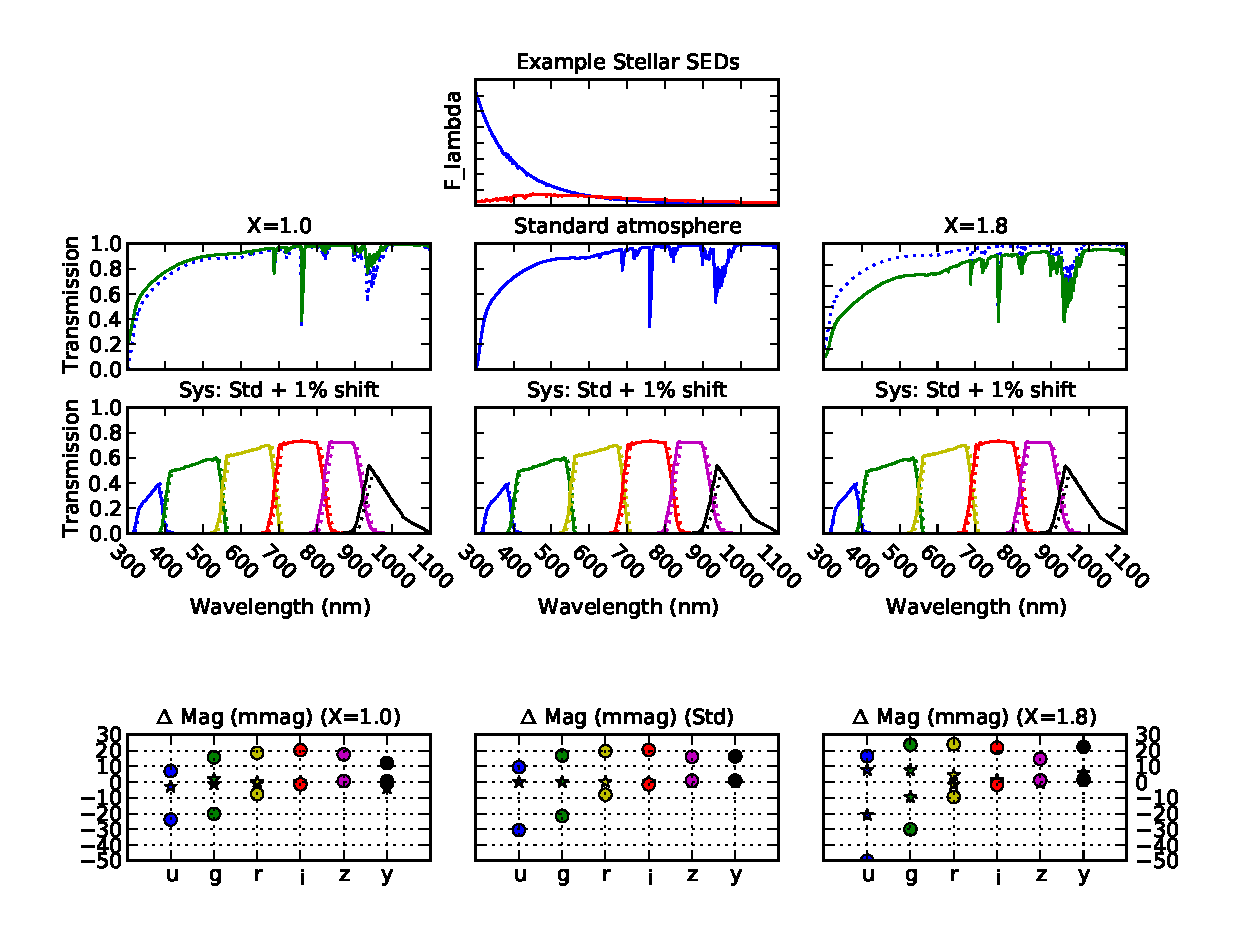
\includegraphics[width=6in]{delta_mags}
\caption{ {\small {\bf Changes in observed magnitudes (counts) due to variations in
hardware and atmospheric bandpass shape.} Two main sequence kurucz model
stars, one blue (35000 K) and one red (6000 K), were used to generate
observed magnitudes (equivalent to $-2.5\, log(C_b)$ - the counts in
Eqn~\ref{eqn:counts}) using three different atmospheric transmission
profiles and two different hardware transmission profiles. The stellar
flux profiles are shown in the top center panel, while the atmospheric
transmission functions ($S^{atm}(\lambda)$) are shown across the
second row and the two hardware transmission profiles
($S_b^{sys}(\lambda)$) are duplicated across the third row. The
atmospheric transmission profiles correspond to an airmass=1.0, 1.2
and 1.5 (from left to right), with variable atmospheric absorption
components. The X=1.0 atmosphere is very similar but not
identical to the current LSST default X=1.2 atmosphere throughput
curve, which is used as `standard' here. The hardware transmission
profiles consist of a `standard' profile (matching the LSST current
expected values) and version where the filter throughputs have been
shifted by 1\% of the effective wavelength of each filter (consistent
with the shift expected near the edge of each filter). The final row
demonstrates the changes in observed magnitudes produced by the X=1.0,
`standard' and X=1.5 atmospheres (left to right, respectively),
combined with both the `standard' hardware transmission (represented by
the star points) and the +1\% shifted hardware transmission (represented
by the filled circles) for both the red and blue stars. The exact
differences in magnitudes resulting from this calculation are listed in
Table~\ref{tab:delta_mags}. }
\label{fig:delta_mags} }
\end{figure}

\begin{center}
\begin{table}[htb]
\caption{{\bf Changes in observed magnitudes due variations in system and atmospheric
 bandpass shape (see also Fig~\ref{fig:delta_mags}) } }
\begin{tabular}{l l | c c c c c c}
& & $u$ & $g$ & $r$ & $i$ & $z$ & $y$ \\ 
\hline \hline
Standard atm, std sys  &  red & 21.472 & 20.378 & 20.000 & 19.911 & 19.913 & 19.913 \\
Standard atm, std sys  &  blue & 19.102 & 19.503 & 20.000 & 20.378 &
20.672 & 20.886 \\ \hline \hline
& & \multicolumn{6} {c} {{\small Change in observed magnitude due to bandpass
shape }} \\ 
\hline
Standard atm, +1\% sys shift & red  & -0.031 & -0.022 & -0.008 & -0.002 & 0.001 & 0.001 \\
Standard atm, +1\% sys shift & blue  & 0.009 & 0.017 & 0.020 & 0.020 & 0.016 & 0.016 \\ \hline
X=1.0, std sys & red  & 0.003 & -0.000 & 0.000 & -0.000 & 0.000 & 0.001 \\
X=1.0, std sys & blue  & -0.001 & 0.000 & -0.001 & -0.000 & -0.001 & 0.005 \\ \hline
X=1.0, +1\% sys shift & red & -0.028 & -0.022 & -0.008 & -0.002 & 0.001 & 0.002 \\
X=1.0, +1\% sys shift & blue & 0.008 & 0.017 & 0.019 & 0.020 & 0.014 & 0.021 \\ \hline
X=1.5, std sys  & red & -0.012 & -0.004 & -0.001 & -0.000 & -0.000 & -0.000 \\
X=1.5, std sys  & blue & 0.005 & 0.003 & 0.002 & 0.001 & 0.001 & -0.000 \\ \hline
X=1.5, +1\% sys shift & red & -0.042 & -0.025 & -0.009 & -0.002 & 0.001 & 0.001 \\
X=1.5, +1\% sys shift & blue & 0.014 & 0.019 & 0.022 & 0.021 & 0.017 & 0.016 \\ \hline
\end{tabular}
\label{tab:delta_mags}
\end{table}
\end{center}

\begin{figure}[htbp]
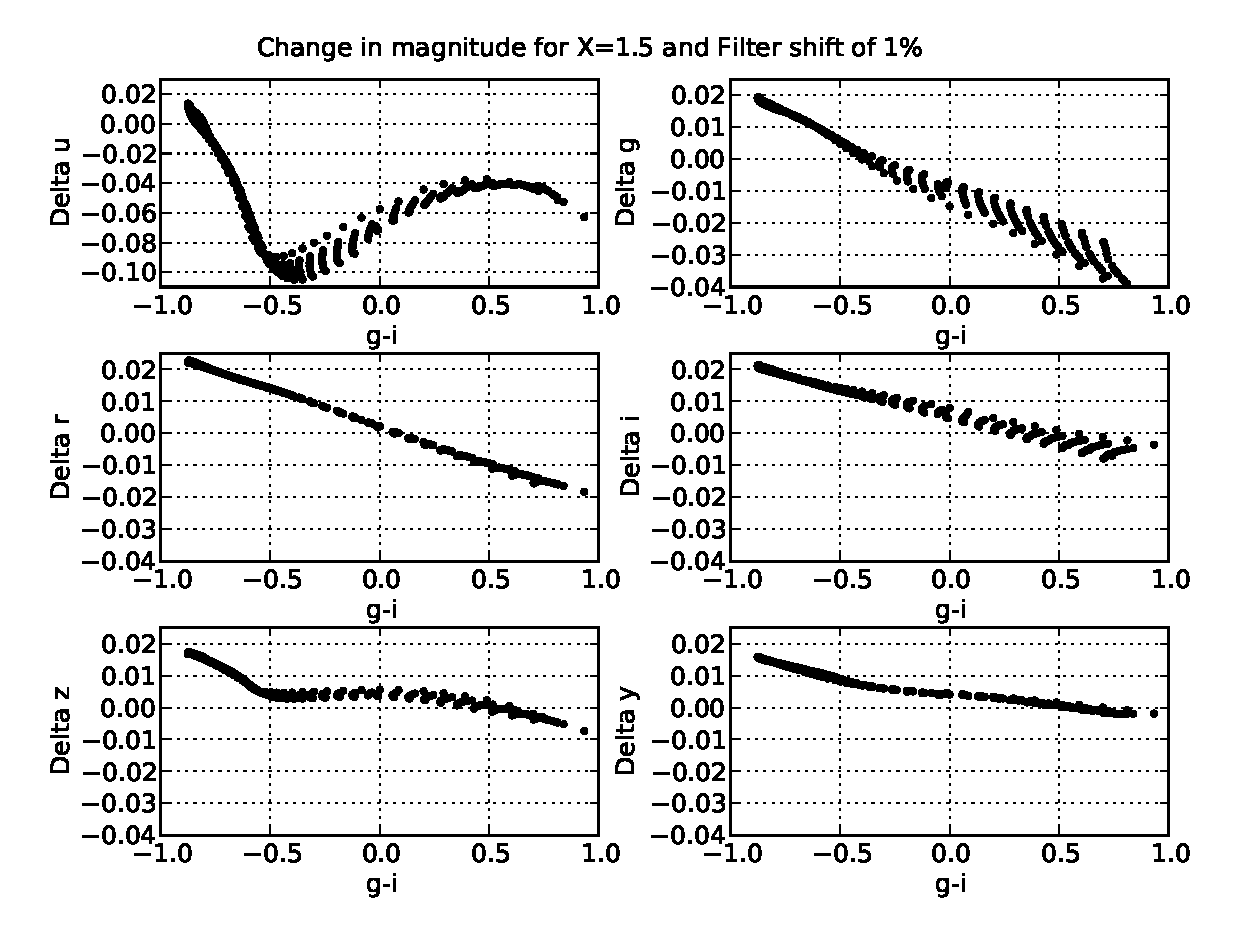
\includegraphics[width=6in]{delta_mags2}
\caption{ {\small {\bf Changes in observed magnitudes (counts) due to a
change in bandpass shape corresponding to a filter shift of $1\%$ and
an $X=1.5$ atmosphere.} 850 Kurucz models with temperatures between
5000K and 35000K and metallicity indexes between -5.0 and 1.0 (solar)
were combined with a standard system response (standard atmosphere and
standard hardware bandpasses), then with a total system response where
the atmosphere was replaced by an X=1.5 atmosphere and the filter
component of the hardware transmission was shifted by 1\% (similarly
as in Fig~\ref{fig:delta_mags}).  It can be seen that the relationship
between $\Delta m$ and $g-i$ can be parameterized, although generally
not with a simple linear relationship. In some cases (such as seen in
the $\Delta u$ and $\Delta g$ panels), calculating $\Delta m$ to SRD levels may
require more than a simple $g-i$ color, but this is then primarily a 
function of metallicity which is possible to determine given the $u-g$ color
in addition to the $g-i$ information. The points in each plot are color-coded
by metallicity, in steps of 1 dex between -5.0 (blue) to 1.0 (magenta).}
\label{fig:delta_mags2} }
\end{figure}


\subsection{From counts to photons}
\label{sec:counts2photons}

The previous section laid out the origins of ADU count variability
from one observation to another. Now we will consider how we can, in
practice, acquire the information necessary to convert a particular
observed ADU count to a measurement of $F_\nu(\lambda,t)$ above the
atmosphere for a particular object.  In other words, how we can
recreate the `truth' by compensating for the variations in
$S^{atm}(\lambda,alt,az,t)$ and $S_b^{sys}(\lambda,x,y,t)$, using the
separability of the normalization and shape of the total system
response.

Let us first consider measurement of the variations in
$S_b^{sys}(\lambda,x,y,t)$.  By using a dome-screen system that is
capable of producing light at a range of individual wavelengths, we
can measure the sensitivity of the hardware (mirrors + lenses + filter
+ detector) transmission as a function of $x$,$y$ at each wavelength,
producing a data cube of `narrow band flat fields'. At a particular
$x,y$ location, this data cube records the shape of the transmission
response in $\lambda$ (measuring $\phi_b^{sys}(\lambda,t)$). By
flattening the data cube through the $\lambda$ axis using a chosen
spectral energy distribution, the resulting 2-dimensional ($x,y$)
`synthetic flat field' records the normalization of
$S_b^{sys}(x,y,t)$. Generation of the synthetic flat field in this
manner is time-consuming (requiring many hours to scan through all 6
filters at the necessary wavelength intervals, $\sim1nm$), however the
wavelength-dependent effects are expected to vary only slowly over
time, so the full narrow band flat field scan will only be repeated
every 30 days. Since gray-scale normalization changes are likely to
occur on a much more rapid timescale, standard white-light flat fields
will also be acquired at the start and end of each night. These
will be used to correct the normalization of the system response on a
nightly basis, updating the synthetic flat field (which has the
desired SED) for the current changes in normalization. This flat field
correction is particularly important over small spatial scales, as no
later calibration stage can contribute to normalization corrections at
less than a few times the Point Spread Function (PSF).

It is worth noting that these flat fields (both narrow band and
white-light) must themselves be corrected for the effects of pixel
scale variations across the field of view, for ghosting caused by
internal reflections in the camera and for the presence of stray or
scattered light captured in the flat. This correction is called the
`illumination correction'. The illumination correction will be
generated by combining the measurements of the system throughput from
the dome screen narrow band flats, measurements of bright, dense star
fields rastered across the field of view during specialized observing
sequences, and measurements of the ghost patterns at various
wavelengths and incident angles obtained with the `camera calibration
optical bench' (CCOB).  It is likely (as the ghosting pattern is
wavelength-dependent) that this illumination correction will have some
wavelength dependence. See Figures~\ref{fig:flatfield} and
\ref{fig:iceffect} for a visual example of the illumination correction
and effect on image processing. The illumination correction is expected 
to be stable with time and will be remeasured only when the optical path
of the telescope is altered. 

Next, considering $S^{atm}(\lambda,alt,az,t)$, we will again separate
the measurement of the shape of the atmospheric response and the
measurement of normalization of the transmission.  The
wavelength-dependent variations in $\phi^{sys}(\lambda,t)$ change
smoothly over spatial scales larger than the field of view and over
several minutes.  By using an auxiliary telescope equipped with a
spectroscope to observe bright stars with known SEDs, we can measure
atmospheric absorption at a variety of positions in the sky every
5--10 minutes throughout the night. These observations are used as
constraints for MODTRAN atmospheric models, generating simpler
representations of the atmospheric throughput (in the form of a set of
absorption components as a function of $alt,az,t$). These components
can be interpolated to generate a wavelength-dependent atmospheric
absorption profile, $S^{atm}(\lambda,alt,az,t)$, for each
observation. In order to correct for the higher frequency gray-scale
variations in the normalization of $S^{atm}(alt,az,t)$ due to cloud
extinction, we must use the observations of stars in the images
themselves, as the cloud extinction can vary up to 0.01 magnitudes on
the scale of a CCD \citep{Ivezic2007} as fast as a few minutes. This
`self-calibration' procedure could be thought of as creating a massive
calibration `standard' star catalog, where the calibration stars are
all of the non-variable, main-sequence stars in the science images;
the main difference is that the true magnitudes of the calibration
stars have to be bootstrapped from the many different observations of
the survey. The calculation of the calibration star magnitudes and
the determination of the normalization for $S^{atm}(alt,az,t)$ are
achieved simulataneously. First the previously described corrections
for $\phi^{atm}(\lambda,t)$, $\phi_b^{sys}(\lambda,t)$ and the flat
field normalization must be added to each observation, producing a
`standardized' magnitude for each star, and then in
`self-calibration', we minimize the difference between the
standardized magnitude and a model magnitude,
\begin{equation}
\label{eqn:chi2}
\chi^2 = \Sigma_{ij} \left( { m_{b,ij}^{std} - m_{b,ij}^{model} \over \sigma_{b,ij}^{std} } \right)^2
\end{equation}
where the model magnitude is derived from the best-fit `true'
magnitude of the calibration star and the normalization constant
(zeropoint offset) for this `patch' (equivalent to the size of a CCD)
\begin{equation}
m_{b,ij}^{model} = m_{b,i}^{best} - \delta z_{b,j}.
\end{equation}
This produces best-fit magnitudes for the calibration star catalog as
well as zeropoint offsets (normalization constants) for each CCD in
every observation. This procedure can also correct for variations in
the normalization of the total system throughput beyond those
contributed by cloud extinction, but will not be sensitive to changes
on scales smaller than a patch.  This is similar in nature to the
ubercal method applied to SDSS in \citet{Padmanabhan2008}.

Using Equation~\ref{eqn:counts}, we can define a `natural magnitude'
\begin{eqnarray}
\label{eqn:defnatmags}
m_{nat} & = & -2.5 log_{10} \left( \int_0^\infty
   {F_\nu(\lambda,t)\phi_b^{std}(\lambda)  d\lambda} \right) \\
 & = &-2.5 log_{10} \left( {C_b(alt,az,x,y,t) \over 
{C'}^{atm}(alt,az,t) \, {C'}_b^{sys}(x,y,t) \,
K'{\textbf(} \int{ f_\nu \phi_b^{obs} d\lambda}{\textbf)} } \right) \nonumber \\
\end{eqnarray}
describing the quantity we wish to derive from the measured ADU
counts.  The natural magnitudes can be related to the corrections 
just described above by 
\begin{eqnarray}
\label{eqn:defnatmags2}
m_b^{nat} & = &-2.5 \, log_{10} \, (C_{b, raw}(alt,az,x,y,t))
\nonumber \\ 
 & & +\, \delta z_b^{ff}(x,y,t) + \, \delta z_b^{selfcalib}(alt,az,t)  \nonumber \\ 
 & & +\, \delta k_b^{atm+sys}(alt,az,x,y,SED,t), 
\end{eqnarray}
where $\delta z_b^{ff}$ comes from the normalization constant derived
from the illumination-corrected synthetic flat field, updated for
variations in normalization on a night-to-night basis by the
white-light flat (and applied directly to the science images at the
pixel level in the traditional manner), $\delta z_b^{selfcalib}$ comes
from the normalization constant derived from the self-calibration
method, and $\delta k_b^{atm+sys}$ depends on the shape of the total
system response (atmosphere + hardware measured from the auxiliary
telescope and the narrow band flat fields) as well as the shape of the
source SED. The color-term correction $\delta k_b^{atm+sys}$ is
effectively a lookup table for each observation, where
$\phi_b^{sys}(\lambda,x,y,t)$ and $\phi^{atm}(\lambda,alt,az,t)$ are
combined with a series of model SEDs and the resulting magnitude
variation is recorded as a function of source SED and $x,y$ in the
focal plane (as the atmospheric variation is roughly constant across
the field of view). For many sources (but not calibration stars) LSST
will simply assume a flat SED, at which point the $\delta
k_b^{atm+sys}$ correction becomes zero, and users may create their own
SED and correction tables based on their knowledge of the true SED
(see Appendix~\ref{sec:photo_better}).

These natural magnitudes are calibrated for variations in the
observed bandpass shape (where applicable) and normalization, thus are directly
comparable from one observation to another. However, they are not tied
to an external physical scale (or from one filter to another), and
thus only define an internally calibrated LSST magnitude in a
particular filter.

To fulfill SRD requirements ~\ref{color_req} and ~\ref{abs_req}, these
internally calibrated natural magnitudes must be tied from one filter
band to another, and then tied to an absolute external physical scale.
For this, a further set of measurements is needed. In all filters, a
set of objects with a well-known spectral type (such as main sequence
stars or white dwarfs, preferably with direct observations of the SED
of the specific object) must be observed and calibrated, in individual
filters, as above. The prior knowledge of each SED is combined with
the standard bandpass shape to generate synthetic color
photometry. These synthetic colors are then compared with the
calibrated measured natural magnitudes to calculate $\Delta_{b-r}$,
the corrections needed to tie measurements in each filter together
(referenced to $r$ band).  At this point, only one final measurement
is necessary to tie the entire system to an external physical scale:
an $r$ band LSST natural magnitude measurement of an absolutely
calibrated source on a photometric night. Although in theory these
last two steps could be done with a single externally calibrated
object, on a single photometric night, a larger set of external
reference objects with well known AB magnitudes will be used to reduce
systematic errors. This defines an AB magnitude,
\begin{equation}
\label{eqn:extmags}
m_b^{AB} = m_b^{nat}  + \Delta_{b-r} + \Delta_r
\end{equation}
which can be compared to absolute physical flux scales. 

The sequence for photometric calibration is then:
\begin{enumerate}
\item{Acquire narrow band flat fields on a monthly basis, acquire
white-light flat fields to update the narrow band flat fields on a
nightly basis, and generate an illumination correction on a
many-monthly basis. Apply the illumination correction to the narrow
band flat fields and combine the narrow band flat fields into a
synthetic flat using a chosen SED (perhaps mimicking the night sky
SED). Scale the synthetic flat for any measured changes in the
white-light flat occuring since the generation of the synthetic
flat. Apply final synthetic flat to images directly, dividing science 
images by the synthetic flat field.}
\item{After remaining image processing (bias correction, fringe correction, etc)
extract ADU counts of sources from images. }
\item{Acquire spectra of known stars on a 5--10 minute timeline
throughout each night, fit for atmospheric absorption coefficients 
and generate atmospheric response curve for each science image's
$alt,az,t$ based on MODTRAN models, retrieve hardware
response curve from narrow band flat fields at various $x,y$ locations
within the focal plane. Using a range of model SEDS, generate a table
of $k_b^{atm+sys}(x,y,SED)$ corrections for each observation. Apply
$k_b^{atm+sys}$ corrections to stars chosen for self-calibration.}
\item{At appropriate intervals (such as at Data Release), minimize
$\chi^2$ from Equation~\ref{eqn:chi2} for the self-calibration stars
and record $\delta z_b^{selfcalib}$ for each patch (each CCD in each
observation).}
\item{Apply $\delta z_b^{selfcalib}$ to all stars in calibration
patch. If an SED is known or has been chosen for particular science
targets, apply appropriate $k_b^{atm+sys}$ correction.}
\item{Apply measured corrections $\Delta_{b-r}$ and $\Delta_r$.}
\end{enumerate}
resulting in calibrated $m_b^{AB}$ values in a standardized bandpass shape, 
with above-the-atmosphere fluxes. 

\section{The internal calibration process}
\label{sec:calib_details}

The next subsections expand on each of the internal calibration steps
leading to natural magnitude measurements described above, including
how each correction is measured, calculated and applied.  These steps
described in this section are applied to each filter
independently. The end result of the internal calibration process is a
set of natural magnitudes, $m_b^{nat}$, measured for each object in
each visit, together with a record of $\phi_b^{sys}(\lambda,x,y,t)$
and $\phi^{atm}(\lambda,alt,az,t)$ (the shape of $S_b^{sys}$ and
$S^{atm}$), the flat field applied (normalization of $S_b^{sys}$), the
zeropoint offset calculated for cloud extinction (normalization of
$S^{atm}$) and the spectral energy distribution assumed for the object
to calculate $m_b^{nat}$ (which may be a flat SED, in which case
$m_b^{nat}$ only includes normalization corrections).

\subsection{Normalization of the hardware transmission}
\label{sec:narrowband}

Compensation for variations (in $x,y,t$) in the normalization of the
hardware transmission ($S_b^{sys}$) will be done using a flat field measured
using narrow band and white light flat fields, after these are
corrected for differences in illumination patterns between the dome
screen and the night sky (the `illumination correction'). This is the
first step in photometric calibration and is necessary to correct for
variations in the normalization of $S_b^{sys}$ that are smaller than a
few times the PSF (and in the current calibration implementation,
smaller than the scale of a CCD).

The specialized hardware for this flat field measurement is an array
of projectors mounted in the dome of the LSST enclosure instead of the
traditional `dome screen'. These projectors will be illuminated with
both broadband (e.g. quartz lamp) and tunable narrow band (essentially
monochromatic) light sources.  Adjustment of the wavelength of the
tuneable narrow band light source can be as fine as 1~nm. The
projectors are designed to fill the LSST etendue with a uniform
illumination, smoothly varying by less than 1\% across the camera
field of view (corresponding to less than 10\% variability across the
projector surface) and less than 0.25\% on scales smaller than
$0.5^{\circ}$ (a little larger than the size of a CCD).  The
projectors will also be designed to limit the extent of light emitted
outside the range of angles seen by the camera to reduce stray light
in the flat fields \citep{Gressler2010}. A set of precision diodes
will be used to normalize the photon flux integrated during flat field
exposures, thus allowing a precise comparison of the system response
at different wavelengths when using the narrow band light sources.
These photodiodes, together with their read-out electronics, will be
calibrated at the U.S. National Institute of Standards (NIST) to
$\approx0.1\%$ relative accuracy across wavelengths from 450~nm to
950~nm. The response of these diodes varies smoothly across this range
of wavelength and provides a well-behaved reference for determination
of $S_b^{sys}(\lambda)$.  Further details of the LSST narrow band flat
field apparatus can be found in \citet{Gressler2010}.  Preliminary
results from a similar apparatus tested at PanSTARRS can be found in
\citet{Stubbs2010a}, as well as earlier experiments from CTIO described
in \citet{Stubbs2007a}.

In each filter, a set of narrow band flats will taken at a series of
wavelengths to form a data cube of flat fields in
($x,y,\lambda$). Using the photodiode measurements of the light
emitted at each wavelength, the data cube can be collapsed to a single
`synthetic flat field' image ($x,y$) by choosing a desired spectral
energy distribution, then combining the individual narrow band images
after applying an appropriate illumination correction (see
subsection~\ref{sec:ic} for details on the illumination correction) for each
wavelength and weighting by the goal SED and the photodiode
measurements. The desired SED could be a single, constant SED or could
be a set of SEDS, but will be clearly defined during the commissioning
period. One choice might be a night sky SED to match the majority of
pixels in each image; the goal SED would then vary throughout the
lunar cycle.

\begin{figure}[htbp]
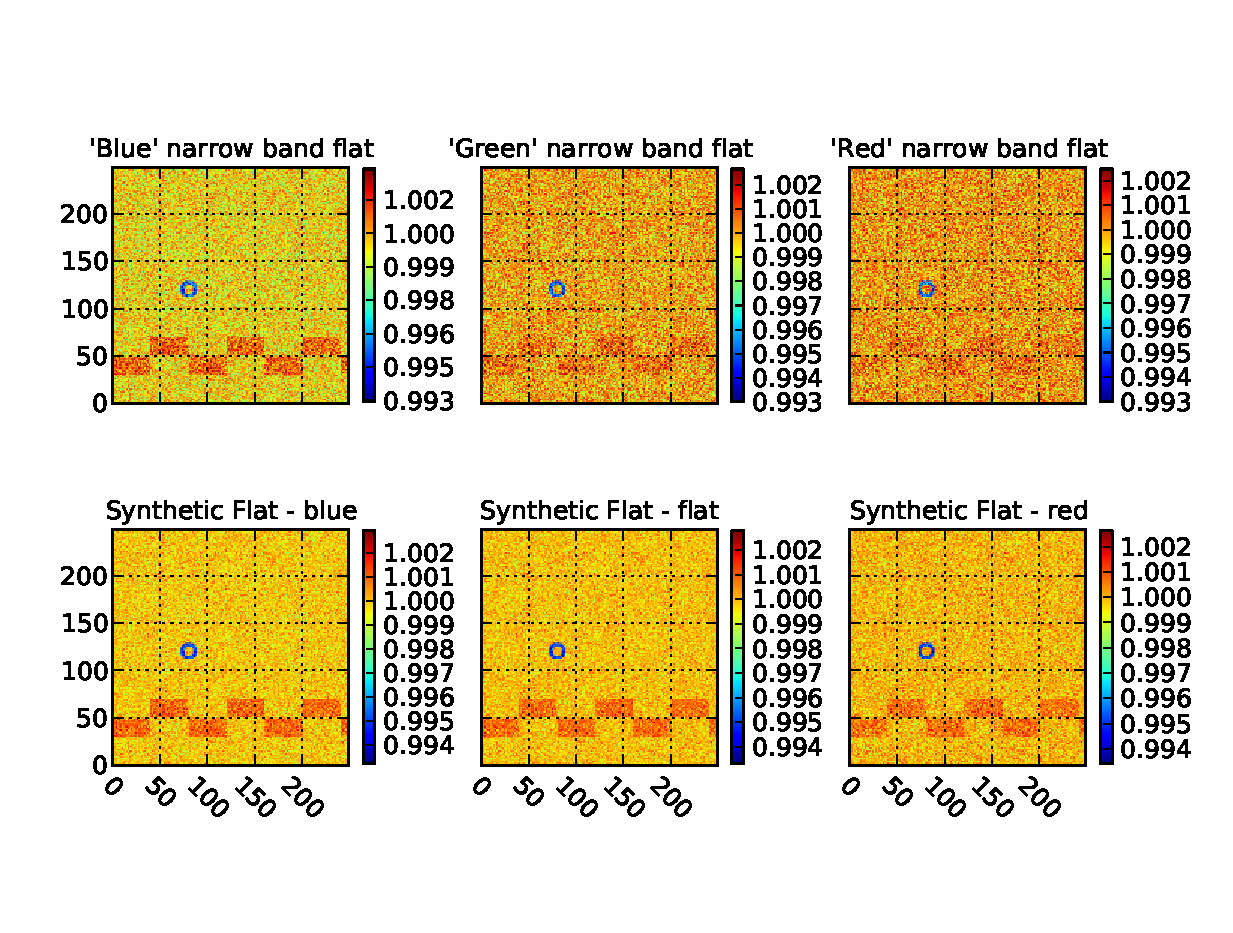
\includegraphics[width=6in]{narrowband_flat}
\caption{ {\small
{\bf Simplified examples of synthetic flat generation.} 
The top panel illustrates simplified narrow band flats, at 'blue',
'green' and 'red' wavelengths. These represent illumination corrected
(thus the relatively flat illumination pattern!) narrow band flat
fields, where the detector shows a sensitivity pattern that is more
pronounced in the blue wavelength flat field. The bottom panel shows
the result of combining these flats to create a synthetic flat with a
desired SED that is either weighted toward blue wavelengths (1.5*blue
+ 1.0*green + 0.5*red), a completely even distribution, or a synthetic
flat weighted toward red wavelenghts (0.5*blue + 1.0*green + 1.5*red).
In operations, the synthetic flat will be created using a well-defined
SED that will best correct the system normalization for science
targets in the field. }}
\label{fig:narrowband}
\end{figure}

The narrow band flats are time-consuming to acquire. Scanning through
all 6 filters at 1~nm intervals requires many hours worth of
exposures, but must also be done in minimal levels of ambient
light. Luckily, any wavelength dependent variations in the synthetic
flat are expected to change relatively slowly so the full set of
narrow band flats only need to be acquired approximately once a month,
which could be done during cloudy nights. However, gray-scale
variations in the hardware normalization (due to dust particles on the
filters, etc.) will occur on a much shorter timescale.  Thus, it is
necessary to use a standard white-light flat to correct for these
short timescale gray-scale variations in the system throughput.  The
white-light flat fields will be obtained with the same apparatus as
the narrow band dome flats, but as the number of exposures required to
characterize a filter is dramatically reduced, these white-light flats
can be obtained at the start and end of every night of observing.

The white-light flat is not applied directly to images, as it
does not have the desired spectral energy distribution. Instead,
changes in the white-light flat from night to night will be
transferred to the data cube of narrow band flat fields, adjusting the
narrow band flats for small-scale changes in gray-scale
throughput. This can be done by taking a white-light flat
simultaneously with the acquisition of the narrow band flat data
cube. White-light flats obtained over the next month are compared to
the `simultaneous' white-light flat, and then the narrow band flat
data cube can be multiplied by any observed differences.

The light generated by the quartz lamp must be stable over the time
interval between monthly narrow band flat measurements, to reduce
changes in ghosting or color-dependent sensitivity variations in the
white light flats.

\subsubsection{Generating the illumination correction}
\label{sec:ic}

The ideal flat field would demonstrate the hardware response to a
focal plane illuminated exactly as it would be with a dark night sky,
empty of ghosts, glints, stray or scattered light - recreating the
hardware sensitivity variations across the focal plane as well as the
effects of vignetting, both of which must be accounted for in the
science images. The measured flat field, however, not only contains
the actual vignetting and hardware sensitivity variations but also
variations in the actual illumination pattern of the dome screen
projectors, stray light, ghost images of the dome screen, and the
effect of pixel scale variations across the field of view, which must
be removed using the illumination correction. 

The dome screen projectors will be designed to be uniformly
illuminated to 1\% over the focal plane, but this is already beyond
the SRD specifications for photometric uniformity.  There will be also
light scattered within the camera dewar and some fraction of the light
within the etendue will have undergone multiple reflections within the
camera refractive optics (creating `ghost' images of the light from
the dome screen). Estimates by Photon Engineering, Inc. (Tucson, AZ)
indicate that $\approx1-2\%$ of the light that reaches the camera
focal plane may be stray light that did not originate within the LSST
etendue. In addition, projection effects cause a variation in the
pixel scale from the center to the outer edges of the field of view,
so that the pixels subtending a larger area (the center of the field)
gather more light from the dome screen. This effect {\it is} present
in the night sky science images as well, but does not affect the total
flux measured from astronomical objects, so this gradient must be
preserved in the science images (and thus removed from the flat field
through the illumination correction). 

Illlustrative examples of these effects in a theoretical dome flat and
the corresponding illumination correction are shown in
Figure~\ref{fig:flatfield}, and the effect of this illumination
correct on final measured counts are shown in
Figure~\ref{fig:iceffect}.

\begin{figure}[htbp]
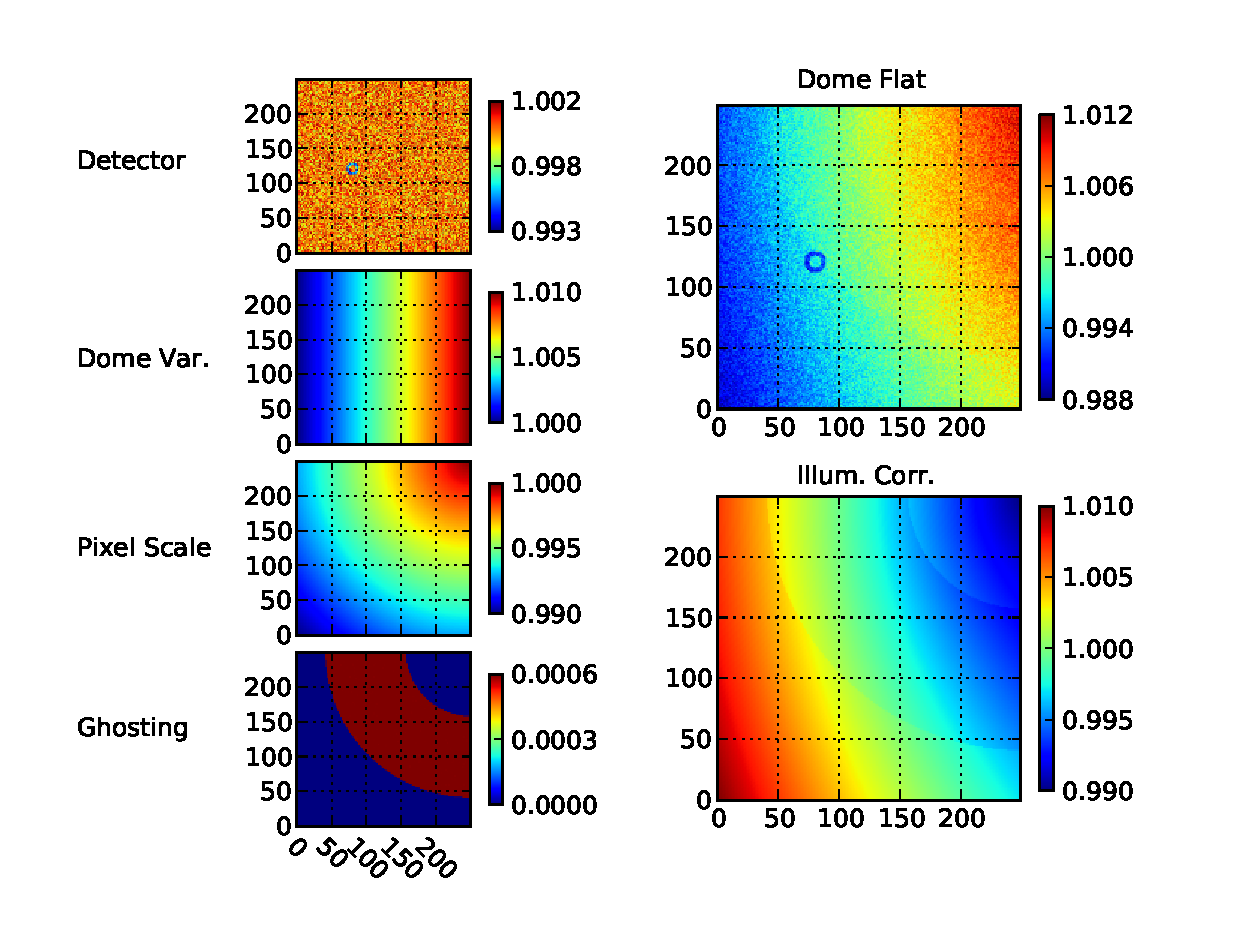
\includegraphics[width=6in]{flatfield_corr}
\caption{ {\small
{\bf Components of the illumination correction.}
Any flat field obtained from the dome screen includes not only a
measurement of small-scale variations in detector sensitivity
(Detector panel, top left), but
also records unwanted effects such as variations in the dome screen
illumination as a function of position (Dome Var. panel), variations in brightness that
result from variations in the amount of sky observed by each pixel
(arising from variations in the pixel scale over the focal plane)
(Pixel Scale panel), and
ghosting caused by internal reflections in the camera (Ghosting panel).
Each panel on the left demonstrates the effect on the total flat field
attributable to each of these variations, in a simplified manner. 
Variations are generated as follows: pixel-to-pixel variation in
detector sensitivity is 0.4\% (as well as a small dust ring), the dome
screen has a 1\% gradient across the field of view, the pixel scale
changes by 0.5\% from corner to corner, and the ghosting is generated
by adding 0.1\% of the total light into a ring reflection. 
The top large panel on the right shows the dome screen flat field that
would be observed after combining all of the effects on the left. The bottom large panel on
the right shows the illumination correction that must be multiplied with 
this flat field to remove the effects of the dome screen variation,
the pixel scale variation, and the ghosting.   Note that no photon noise was
introduced in this simulation. }}  \label{fig:flatfield}
\end{figure}

\begin{figure}[htbp]
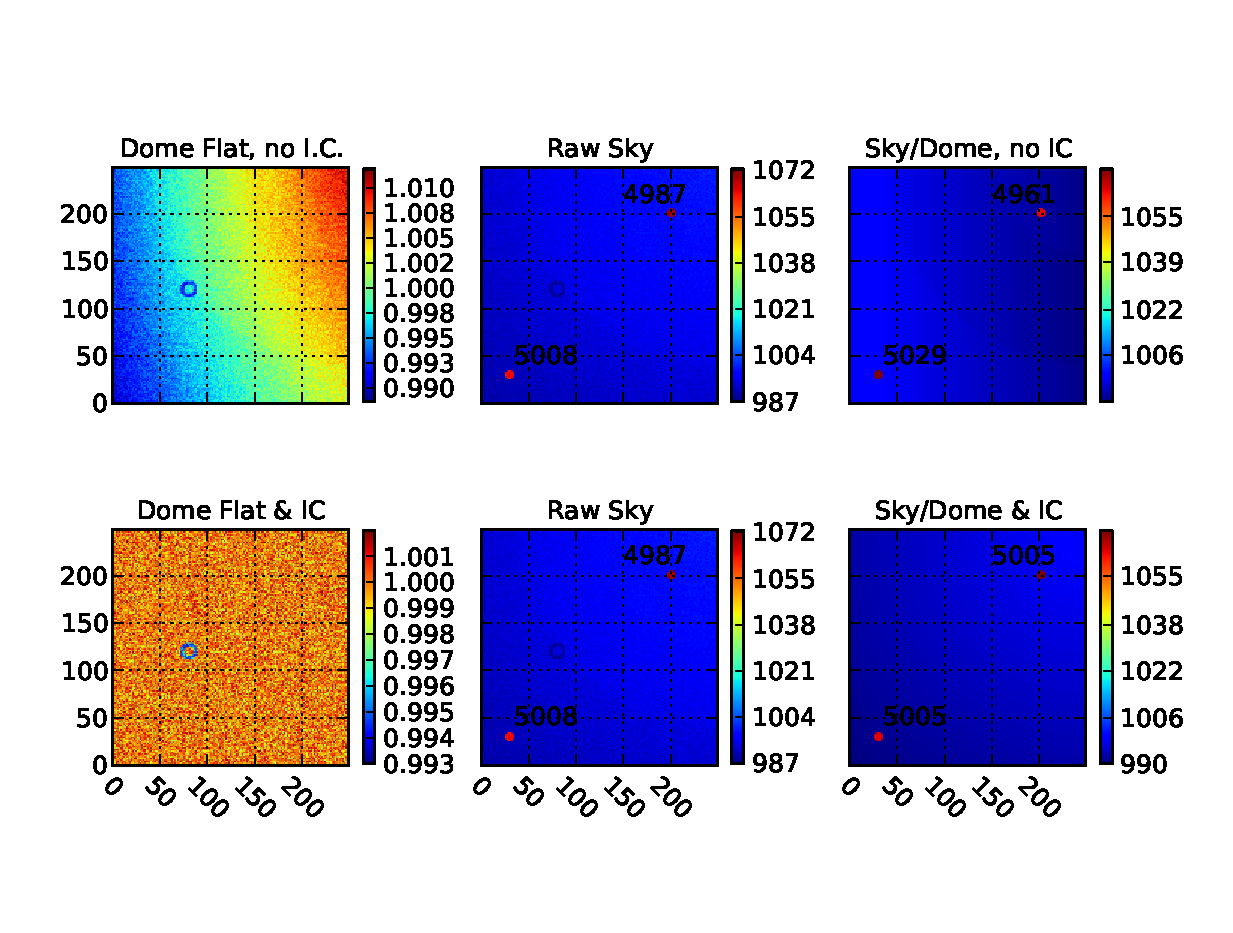
\includegraphics[width=6in]{ICeffect}
\caption{ {\small
{\bf Effect of illumination correction on photometry.}
The left top panel shows a flat field obtained from a dome screen,
creating with the same conditions as in Figure~\ref{fig:flatfield},
without multiplying by an illumination correction. The central top
panel shows a raw `image' of the sky, generated by adding a background
sky value of 1500 counts per pixel (scaled by the pixel area, as in
Fig.~\ref{fig:flatfield}, to two stars. The stars were generated by
placing 5000 counts over a circular aperture the size of the PSF at
the location of the star. A ghost image was created as in
Fig.~\ref{fig:flatfield}.  The right top panel demonstrates the result
of processing the raw sky image by subtracting the ghost image and
then dividing by the dome flat without an
illumination correction. 
The left bottom panel shows the illumination correction applied to the
same flat field. The middle bottom panel shows the same raw sky image as
the top row. The bottom right panel demonstrates an improved processing
of the raw sky image, by subtracting the ghost image and then dividing
by the illumination corrected flat field. 
Note that the sky background does not appear
flat but is correct for preserving stellar photometric accuracy. 
In every image with stars, the numbers next to each star indicate the
counts measured within an appropriate circular aperture for the
star. In the raw images, these counts are not equal because of the
variation in pixel to pixel sensitivities. }} \label{fig:iceffect} 
\end{figure}

Illumination corrections (one per filter) will be generated whenever
the camera is removed from the telescope or the focal path undergoes
significant changes (such as a filter being replaced or the mirrors
being realuminized), but should be stable otherwise. The corrections
will be created by combining information from a ZEMAX model of
ghosting in the camera constrained by measurements from the Camera
Calibration Optical Bench (CCOB), measurements of the observed
individual narrow band dome screen (DS) flats, and dense star fields
rastored across the focal plane on a photometric night.

The first of these components, {\bf Camera Calibration Optical Bench
(CCOB)}, provides a method to calibrate the spatial and
wavelength-dependent response of the focal plane, unmounted from the
telescope, using a well controlled, wavelength-variable, light source
calibrated using a NIST photodiode. This light source, which produces
a spot in the focal plane approximately the size of or smaller than
the PSF, will be scanned across the detector ($x,y$) at a variety of
beam incident angles, ($\theta,\phi$) and at a variety of wavelengths
($\lambda$).  The response of the detector will be measured in two
different configurations: one with only the detector and the dewar
window - which doubles as lens 3 (L3) - and one with the detector, L3,
L2, L1, the filters and the camera shutter. In the L3-only
configuration, the detector response should include only relative
simple ghosting, primarily 3 ghost images from reflections between the
CCD surface and L3. In the full refractive optics configuration (with
L3, L2, L1, the filter and camera shutter), the detector response will
include a more complicated ghost pattern. Current simulations indicate
the strongest ghosts are expected to originate from reflections
between the CCD surface and L3, where the resulting ghosts are
expected to have an amplitude $5\times\approx10^{-4}$ relative to the
flux of the source. Other ghost images, due to reflections between
lens surfaces, should contain about $\approx10^{-5}$ times the flux of
the source.  See Figure~\ref{fig:ghostimage} for an example of
simulated ghosting in the LSST focal plane. These measurements of the
focal plane response in different optical configurations with a known
incoming light source do not directly measure the illumination
correction (for example, neither pixel scale variation due to
projection effects nor the full stray/scattered light from the dome
projectors are included), but it does provide constraints for model
calculations (such as a ZEMAX model) of the illumination pattern in
the camera as a function of wavelength, position in the focal plane,
and beam incident angles, which are necessary for the creation of the
full illumination correction, as well as constrain the focal plane
response itself.

More details about the requirements and physical apparatus of the CCOB
are available in LSST-10015 and LSST-8217.

\begin{figure}
\centering
\includegraphics[width=5.5in,angle=90]{ghost_images}
\caption{ {\small
{\bf Simulations of LSST camera ghost images, as measured by CCOB. }
Various beam incident angles, positions and wavelengths will be
explored by the CCOB, creating focal plane measurements similar to
those simulated above. These measurements will be combined to
constrain a ZEMAX model describing the optical paths in the camera
(including the effect of the actual coating reflectivities of the CCD
and lens surfaces, etc). }}
\label{fig:ghostimage}
\end{figure}

The ZEMAX model describes how light scatters inside the camera
creating ghosts at each wavelength. If the dome screen projectors were
perfectly uniform and no stray light was scattered into the LSST
etendue, the narrow band dome flats plus the predictions from the
ZEMAX model would suffice to create a perfect illumination corrected
synthetic flat. Stray light scattered into the LSST etendue can be
modeled using work similar to that of Photon Engineering, Inc., and
then the model constrained by taking measurements of the focal plane
response while blacking out M2 (to image only the stray light). This
creates a preliminary estimate of the illumination correction, which
is particularly useful for small spatial scales (smaller than a CCD)
which may not be well sampled in the next, rastor-scan step.

To account for illumination variations from the dome screen projectors
on large spatial scales (which could be up to 1\% across the field of
view), stray light scattered from other unmodeled surfaces, or systematic
differences in exposure time due to the camera shutter movement,  a dense
network of stars of a variety of spectral types must be rastored
across the focal plane on a photometric night. The images will be
divided by the synthetic flat field corrected by the preliminary
illumination correction, and then the counts for each star corrected
for varying color terms in the atmosphere and hardware response, as
further described in subsection~\ref{sec:phi_correction}.  The final
update to the illumination correction can then be determined by
minimizing over all stars $i$ in all observations $j$,
\begin{equation}
 \chi^2 =  \Sigma_{i=N_{stars},j=N_{obs}} \left( { m_{ij}^{meas}(x,y) - m_{ij}^{model}(x,y)
\over \sigma_b} \right)^2  
\end{equation}
where the model magnitude of each star in each observation is given by
\begin{equation}
m_{ij}^{model}(x,y) =  m_b,i^{best} - \delta k_{b,j}^{atm+sys}(x,y,alt,az,SED,t) - \int d\lambda \, dZ_{IC}(x,y,\lambda)
\end{equation}
where $m_{b,i}^{best}$ is the best-fit, constant magnitude of the star
in this filter, $k_{b,j}^{atm+sys}$ is the color-term correction
(partially determined by the constant from exposure-to-exposure
hardware throughput curve and partially determined by the varying with
each exposure atmospheric throughput curve), and $dZ_{IC}$ is the
update to the illumination correction which is produced by this dense
rastor scan. Similar applications of rastor scans have been
successfully used in previous surveys, ({\it e.g} \citet{Regnault2009,
Magnier2004, Manfroid1996}), providing an illumination correction
accurate to the sub-percent level. With the additional information
from the CCOB and the better intrinsic uniformity of the dome screen
illumination, we expect the illumination correction for LSST to be at
least factor of 2 more accurate.

\subsubsection{Error in the Normalization of the Hardware Transmission}

The dome screen projectors will be designed to be uniform to bertter than
0.25\% (2.5~mmag) over scales less than $0.5^{\circ}$ (slightly larger
than a CCD). Translating from this engineering requirement (a strict
limit) to the RMS of expected measurements implies a resulting RMS of
0.7~mmag (=2.5~mmag/$\sqrt(12)$) in the dome illumination uniformity
on scales smaller than a CCD. After using the measurements from the
CCOB to model ghost reflections and scattering within the camera, the
uniformity of the dome screen projectors is expected to be the
limiting factor on these small scales. Applying the dense rastor scan
of stars to correct for larger illumination variations from the dome
screen projectors on the scale of the entire field of view, plus to
correct for the effects of 1--2\% stray light and systematic exposure
differences due to camera shutter travel, adds an additional error of
about 2.8~mmag, increasing the expected error in the illumination
corrected synthetic flat field to 2.9~mmag.

The illumination corrected synthetic flats are created on a monthly
basis and then must be updated for gray-scale nightly changes in the
hardware transmission (due to dust,etc) using the white-light flat
fields acquired using the quartz lamp in the dome screen
projectors. As this update only depends on changes in the white light
flats, not their absolute values, the only requirement is that the
quartz lamps produce an illumination pattern in the focal plane which
is stable over time at the same level as the initial illumination
uniformity requirement, or stable to within 0.25\% within a CCD. This
means that the quartz lamps should not change their spectral profile
(which may change the ghosting pattern due to wavelength dependent
effects) or their illumination pattern by more than an amount which
would produce changes of more than 0.25\% in the focal plane, adding a
further 0.7~mmag rms scatter, for a final total of 3~mmag expected
error in the normalization of the hardware throughput.

\subsection{Shape of the Hardware and Atmospheric Response}
\label{sec:phi_correction}

Compensation for the changes in observed magnitudes caused by
variations in the wavelength dependence (shape) of the hardware and
atmospheric response curves, $\phi_b^{sys}(\lambda)$ and
$\phi^{atm}(\lambda)$, will be done using independent measurements of
the hardware response curve (from the narrow band flat fields) and the
atmospheric response curve (from MODTRAN4 models generated from
measurements from the auxiliary telescope).  While the measurement of
the shapes of the hardware and atmosphere curves are independent, the
actual correction that must be applied depends on the combination of
atmospheric and hardware response curves as well as the SED of the
astronomical object.  This correction is necessary for precision
photometry, but as it requires knowledge of the object's SED, most
LSST reported magnitudes will include either no correction or a
(potentially rough) correction along with an indication of what SED
was assumed to generate this value. However, for stars which will be
used in self-calibration (see subsection~\ref{sec:selfcalib}) to
determine photometric zeropoints in each exposure, a model SED
well-matched to the object's colors will be chosen and used to
generate the $\delta k_b^{atm+sys}$ corrections described in this
section.

\subsubsection{Measuring the shape of the hardware response curve}
\label{sec:phi_hardware}

The hardware response curve is measured directly using the individual
narrowband flat fields described in section~\ref{sec:narrowband}. At
each wavelength, the narrowband flat field will be illumination
corrected and then used to measure the total hardware response over
all $x,y$ positions. The dome screen photodiodes will be used to track
the relative intensity of the light produced by the projectors at each
wavelength. These NIST-calibrated photodiodes are expected to be
accurate to within 0.1\% between 400-900~nm ($g,r,i,z$ bandpasses)
with current technology, which can be extended to 1600~nm (into the
$y$ band) using techniques under development (which also have the
possibility of achieving 0.01\% accuracy in the diode calibration at
NIST) \citep{Eppeldauer09}, as shown in Figure~\ref{fig:NIST_diode}. 

\begin{figure}
\centering
\subfloat[\citet{Stubbs2010a}]{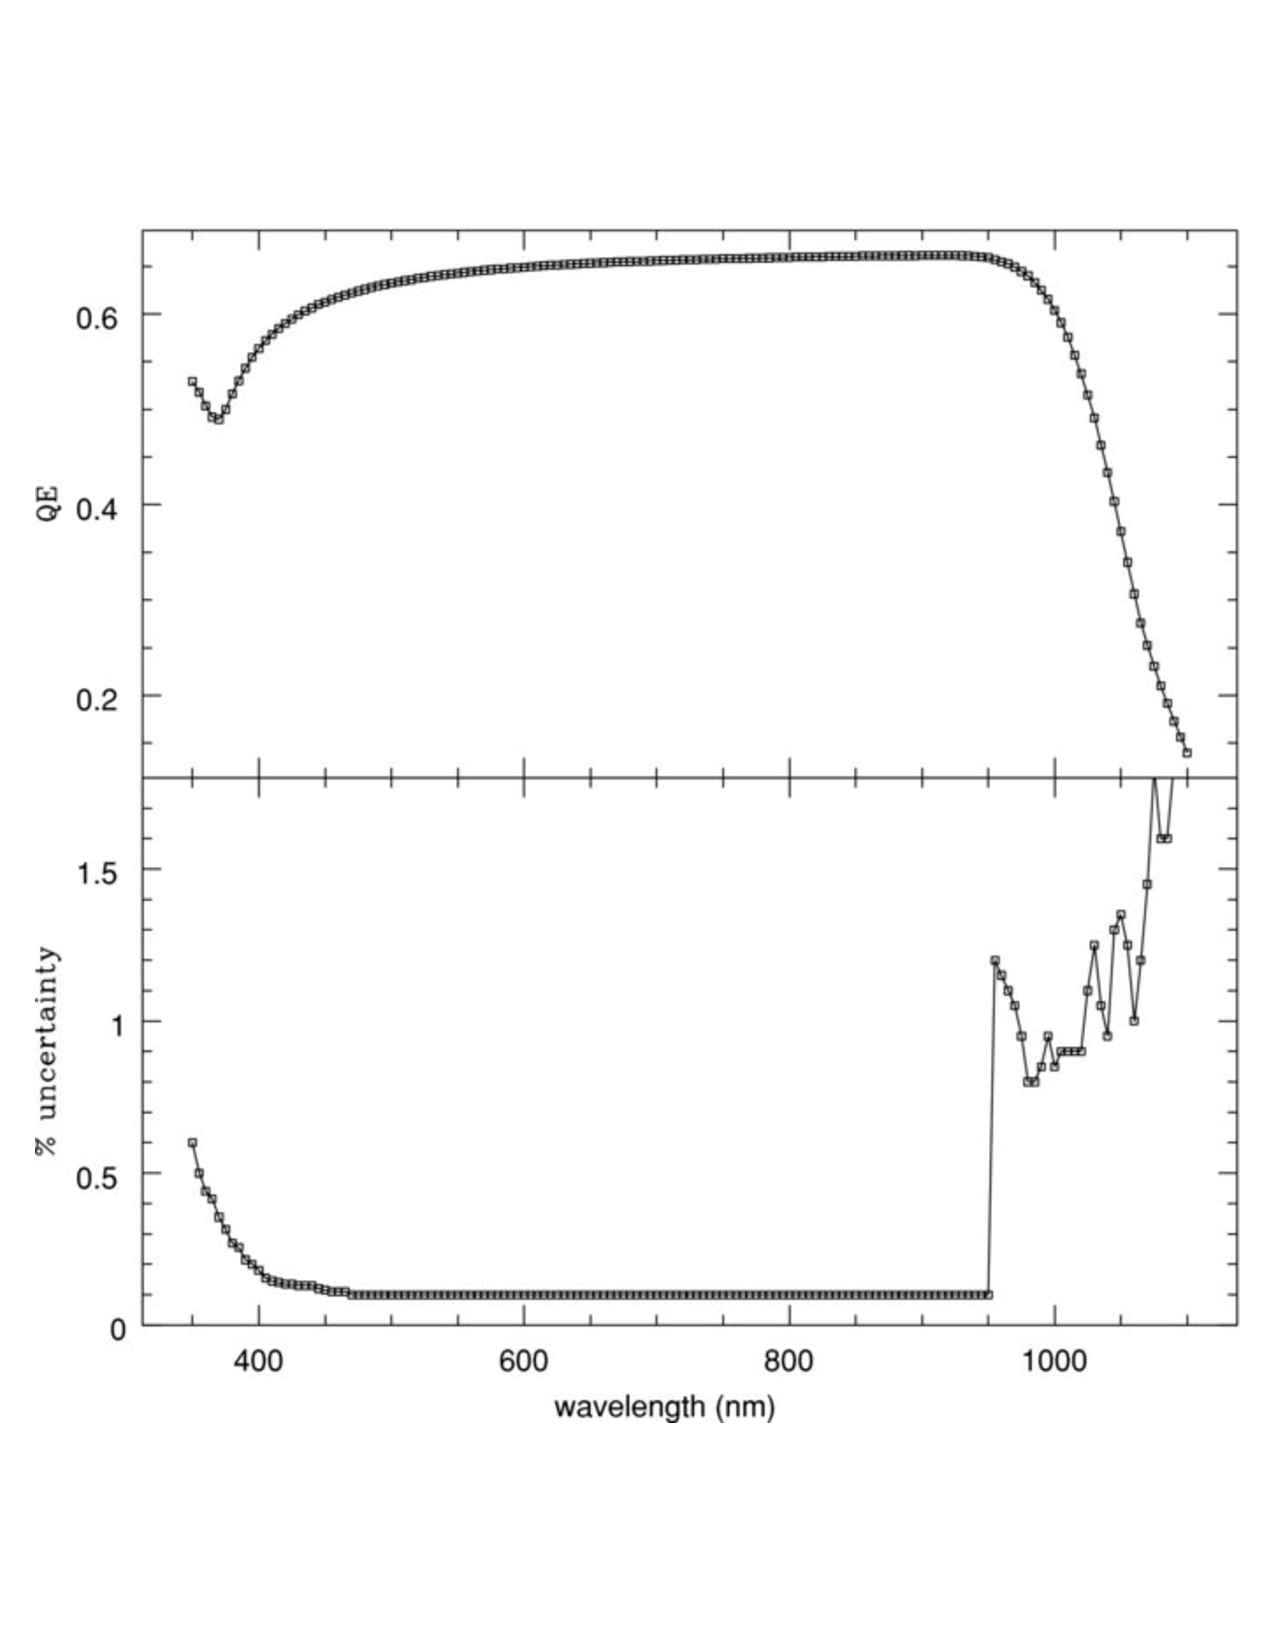
\includegraphics[width=3.5in]{NIST_diode}} \\
\subfloat[\citet{Eppeldauer09}]{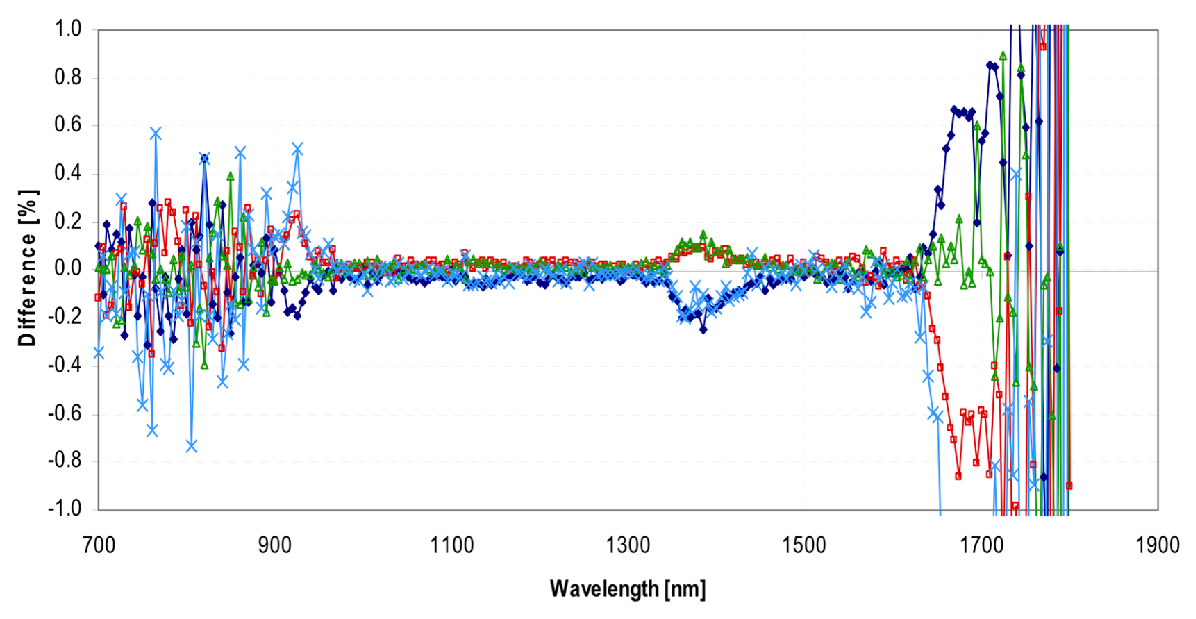
\includegraphics[width=5in]{NIST_diode2}}
\caption{{\small
{\bf Quantum efficiency curve and fractional uncertainty for
NIST-calibrated photodiode, from \citet{Stubbs2010a} and
\citet{Eppeldauer09}.}  Panel (a): Between 400 and 900~nm, calibration
methods already in use in test systems indicate photodiode accuracy is
better than 0.1\%, as in the bottom part of this panel.  The sudden
decrease in calibration accuracy below 900~nm is due to calibration
methods used by NIST in 2005. Panel (b): More recent photodiode
calibration efforts by \citet{Eppeldauer09} show better than 0.1\%
accuracy can be achieved to beyond 1200~nm, the limit of detector
response for LSST, as shown here in the response curves resulting from
multiple scans of a single source using the same photodiode.} }
\label{fig:NIST_diode}
\end{figure}

These measurements will be updated on a monthly basis, as the hardware
response curve is expected to change only slowly over time due to
aging in the filter and mirror coatings. It is expected that the shape
of the response curve will be primarily a function of radius due to
variations in the thickness of the filter coatings caused by the
mechanism used to deposit those coatings. The variation due to filter
nonuniformities is specified to be less than 1\% across the focal
plane, most likely in the form of a bandpass shift as shown in
Figure~\ref{fig:filtershift}. For main sequence stars, the resulting
changes in observed magnitude as the bandpass shifts by 1\% of the
central wavelength can be as much or more than 0.02~magnitudes (20
mmag) - even larger in the $u$ band (see
Figure~\ref{fig:dmag_filtershift}). However, as long as the variation
in the hardware response curve is measured to better than 0.05\% --
equivalent to approximately a 30~Angstrom error in wavelength
calibration of the monochromatic light source throughout the bandpass
or a 0.5\% error in photodiode calibration assuming that the shape of
each bandpass is determined using approximately 100 independent
measurements (i.e. 1 measurement per nanometer within the bandpass) --
the error contribution towards calibrating these observed magnitudes
will be less than 1~mmag for all bandpasses other than $u$, where the
error could be as much as 5~mmag for certain main sequence stars (see
Figure~\ref{fig:dmag_filtershift_small}).

Because the shape of the hardware response curve varies as a function
of filter radius, it is also necessary to monitor any offsets of the
filter position from dead center after any filter changes. Assuming
the filter response curve varies linearly with radius, the filter
location must be measured to better than 0.025\%  for the filter
positioning to remain less than a 0.5~mmag source of error. Given the
filters are approximately 75~cm in diameter, this means the filter 
positioning must be recorded to better than 0.18~mm. 

\begin{figure}
\centering
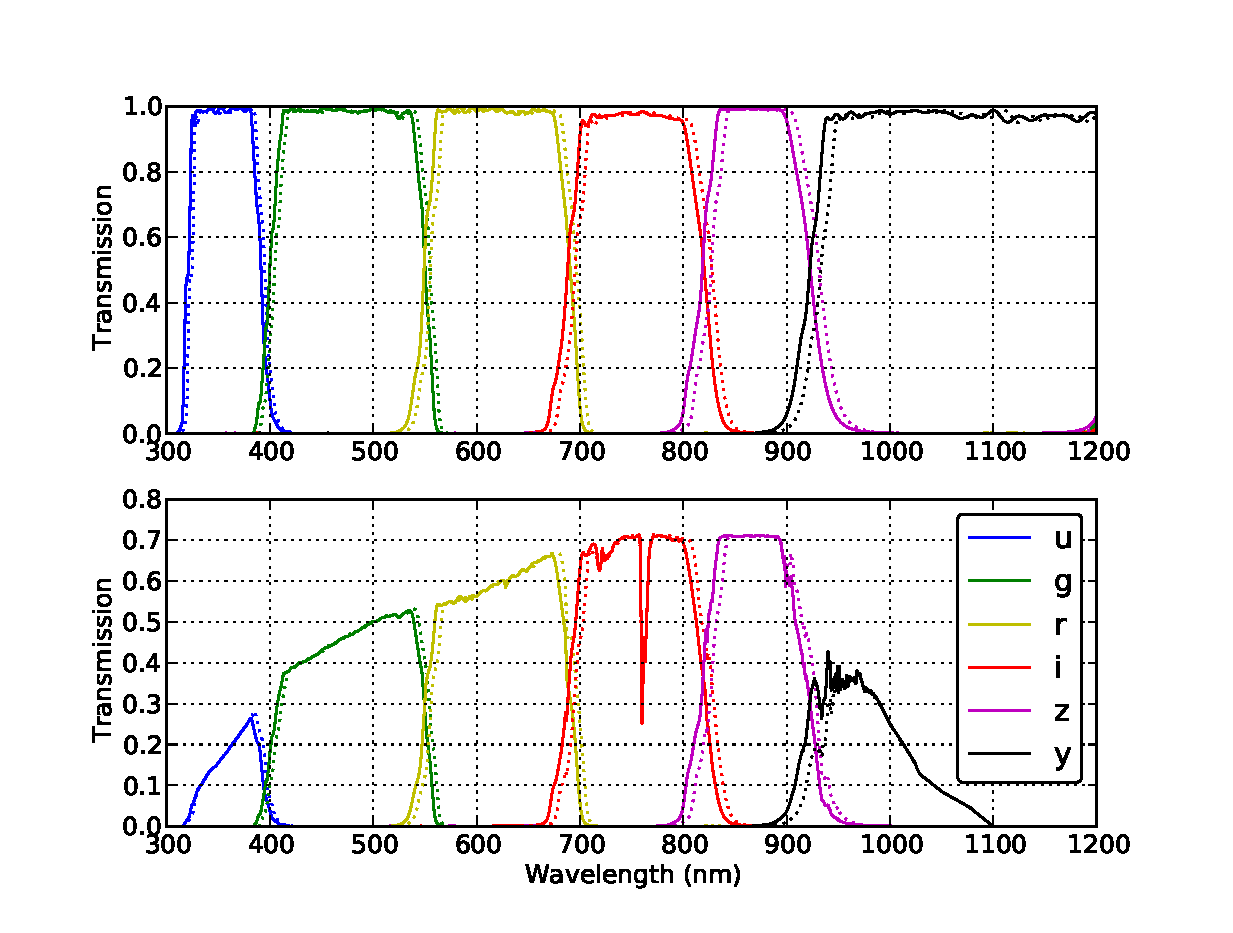
\includegraphics[width=6in]{filter_shifts}
\caption{{\small 
{\bf Baseline filter curves and a potential (1\% of the central
  wavelength) shift due to nonuniformity.}
The solid lines indicate standard filter bandpasses (top panel: filter
alone, bottom panel: filter plus standard mirror, lens, detector and atmosphere
response curves) while the dashed lines indicate the same bandpass
shifted redward by 1\% of the central wavelength.}}
\label{fig:filtershift}
\end{figure}

\begin{figure}
\centering
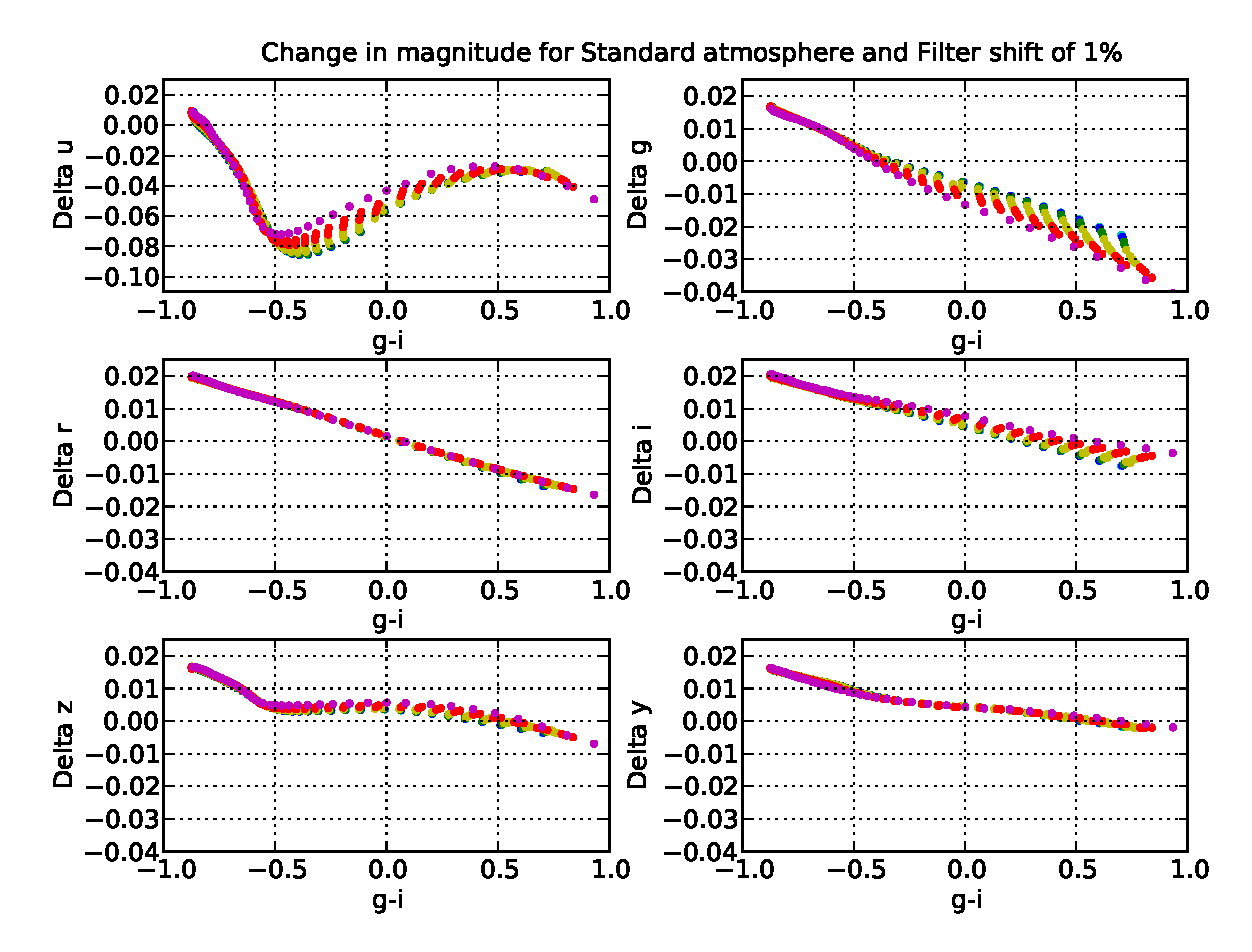
\includegraphics[width=6in]{delta_mags_filtershift}
\caption{{\small 
{\bf Changes in observed magnitude (measured counts)
due to a hardware response curve shift of 1\% of the central
wavelength of each bandpass.}  850 Kurucz models with temperatures
between 5000K and 35000K and metallicity indexes between -5.0 and 1.0
(solar) were combined with a standard atmosphere and standard
hardware bandpass, and then with a total system response where the
atmosphere remained constant but the hardware response was shifted by
1\% of the central wavelength of each bandpass (as in
Fig~\ref{fig:filtershift}).  Changes in magnitude on the order of
20~mmag are typical, except in $u$ band where the shift can create a
$\delta u$ of closer to 80~mmag for certain kinds of main sequence
stars. The points in each plot are color-coded by metallicity, in
steps of 1 dex between -5.0 (blue) to 1.0 (magenta).} }
\label{fig:dmag_filtershift}
\end{figure}

\begin{figure}
\centering
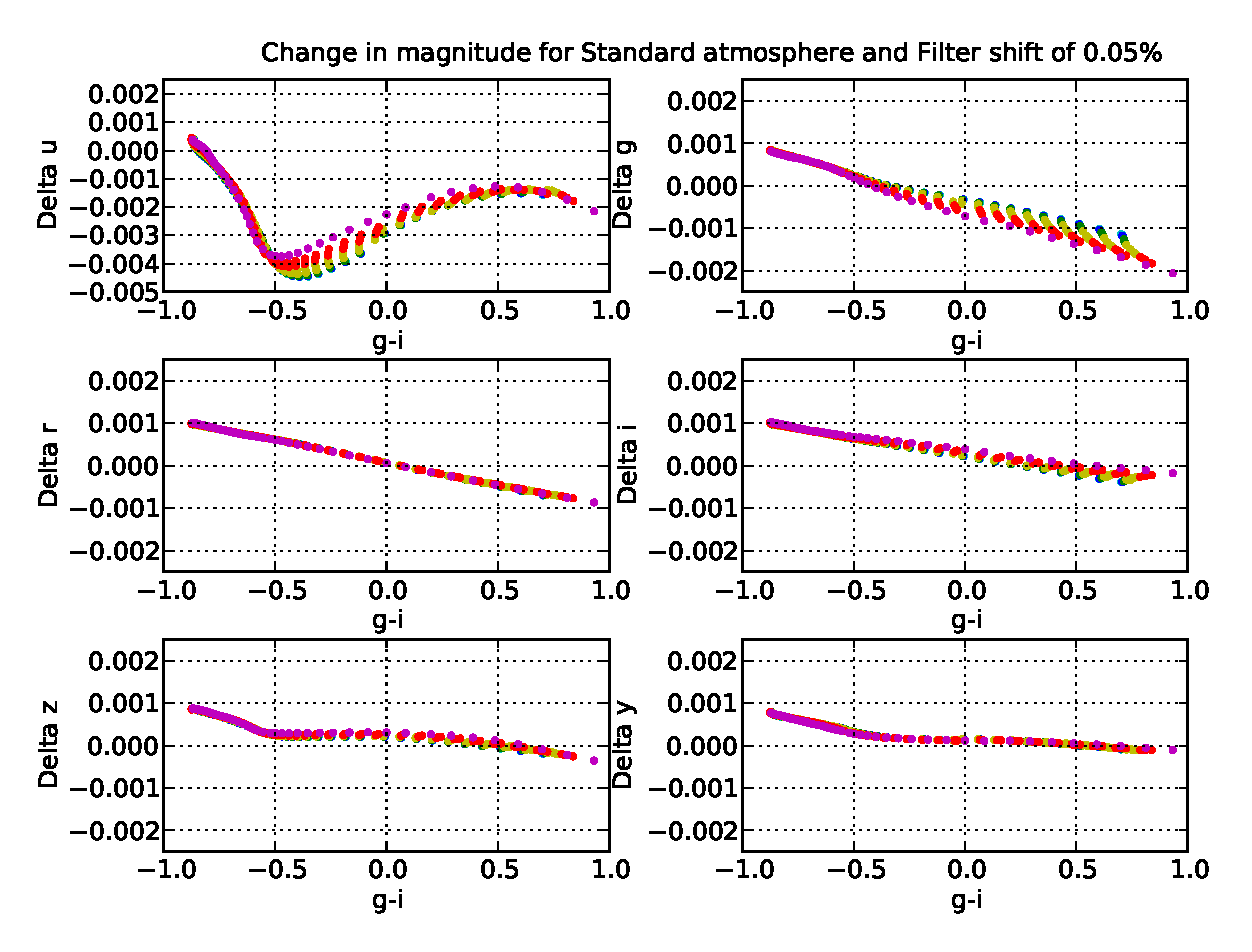
\includegraphics[width=6in]{delta_mags_filtershift_small}
\caption{{\small 
{\bf Changes in observed magnitude (measured counts) due 
to a hardware response curve shift of 0.05\% of the central wavelength
of each bandpass.} Similar to Fig~\ref{fig:dmag_filtershift} except
that the hardware response was shifted by only 0.05\% of the central
wavelength, an amount representing an unmeasured shift in the hardware
response and thus contributing to the final error in the calibration
of the observed magnitudes. }}
\label{fig:dmag_filtershift_small} 
\end{figure}
 

\subsubsection{Measuring the shape of the atmospheric transmission curve}
\label{sec:phi_atmo}

XXX

The atmospheric transmission curve will be interpolated from a series
of spectroscopic measurements of atmospheric absorption generated by 
the auxiliary telescope. It's worth noting that the auxiliary telescope
measurements will not correct for cloud extinction or any other normalization
variation due to the atmosphere; the goal for the auxiliary telescope 
to compensate for changes in the shape of the atmospheric transmission curve.

The atmospheric transmission curve, $\phi^{atm}(\lambda, alt, az, t)$, varies
due to changes 


The spectroscopic measurements from the auxiliary telescope are
necessary to correct for the wavelength-dependent variations in
atmospheric transmission; it is worth noting that these auxiliary
telescope measurements will {\it not} correct for cloud extinction or
any other gray extinction. The wavelength-dependent atmospheric
variations are due to variations in the composition of the atmosphere;
the auxiliary telescope will acquire measurements with a sufficient
sampling rate and spacing across the sky to allow determination of the
atmospheric absorption within each science image, correcting the
`observed' atmospheric transmission curve to the `standard' bandpass.

The auxiliary telescope will be a 1.2m telescope equipped with a
spectroscope which will monitor a set of probe stars as they traverse
the sky each night. The spectra from the auxiliary telescope will be
processed to correct for the efficiency of the spectroscope itself,
leaving the spectra of the star and the signature of absorption from
the atmosphere. The resulting spectra will be fit to state-of-the-art
atmospheric models (such as MODTRAN4 \citep{modtran4a, modtran4b}) to determine
the components responsible for absorption in the spectra, including
molecular scattering, aerosol scattering, and molecular line
absorption from oxygen, nitrogen, ozone and other trace elements, and
specifically absorption from water vapor. The fitted values of these
atmospheric components can then be interpolated to calculate the
atmospheric mix present in any science image, recreating the relevant
$\phi^{atm}(\lambda,alt,az,t)$. Recognition of the atmospheric
components can be done with a relatively modest spectral resolution
(R$\sim400$), but it is important that the full spectral range (300~nm
to 1100~nm) be obtained in a single exposure. Choosing white dwarfs
(with $r<12$) as the probe stars simplifies this procedure as the
white dwarfs have relatively simple spectra, however a range of stars
could be used in which case the spectra of each star can be
bootstrapped from the large number of repeat observations, using an
iterative procedure to extract stellar parameters (effective
temperature and surface gravity) for each of the probe stars along
with the atmospheric constituents.





In addition, the narrow band flats must also be used to measure
changes in the bandpass shape throughout the field of view. Before
applying $\delta k(x,y,SED,t)$ corrections to the observed magnitudes,
however, the wavelength-dependent effects of the atmosphere must also
be considered, as the final effect on the observed magnitude is not
independent. Thus, the narrow band flat fields will be combined using
a series of standard model SEDS to generate $\delta
k(x,y,alt,az,SED,t)$ corrections for each image after the atmospheric
corrections described in Section~\ref{sec:phi_atmo} have been
calculated and applied to the model SEDs. Thus for each observation,
there will be lookup tables created with $\delta k(x,y,alt,az,SED,t)$
that can be parametrized as a function of object color. These $\delta
k$ correct the shape of the system bandpass response to a standardized
value, chosen during commissioning.  Obviously, applying these
corrections requires knowing the color of the astronomical object (and
ideally, the full spectral energy distribution), and this information
will not always be known for all objects. In practice, the calibration
pipeline will calculate corrections using best-estimates of the
objects' color. These estimates will increase in accuracy as the
survey progresses, eventually reaching $\approx 0.07$~magnitudes for
objects with many repeat observations.



By collecting atmospheric absorption measurements every 5-10 minutes 
over a wide range of airmasses and positions in the sky, 

Each interpolated $\phi^{atm}(\lambda,alt,az,t)$, will be combined with
the bandpass shape measured as a function of position in the focal
plane, $\phi_b^{sys}(\lambda,x,y,t)$, as in
Section~\ref{sec:narrowband}), creating a set of $\delta
k(x,y,alt,az,SED,t)$ corrections for each observation.

ADD/CREATE FIGURE showing atmosphere and various components

CREATE FIGURE flowchart? (like figure 4 from calibration preliminary
baseline design?)


\subsection{Normalization of the Atmospheric Transmission}
\label{sec:selfcalib}

After applying each of the previous corrections, the raw counts are
corrected to a `standard' bandpass for each filter,
$\phi_b^{std}(\lambda)$, using both the narrow band flats and the
atmospheric model derived from the auxiliary telescope
observations. Small scale ($<$ several times the PSF) gray-scale
zeropoint variations have also been removed by the synthetic
flat. However, there still remain variations in the normalization of the
system response that result from gray-scale extinction due to
clouds. The self-calibration procedure is necessary to correct for
these zeropoint offsets.

The self-calibration procedure selects bright, isolated main sequence
and white dwarf stars (or any star with well-known colors and a
well-known SED, to reduce errors in the applied
$\delta k$ values) from the sample of all observed stars after they are
corrected to the standard bandpass (`standardized'). Only non-variable stars will be
selected for self-calibration, based on approximately calibrated data
(say, a few percent) which will suffice in this context. It then uses
the many repeat observations $j$ of each star $i$ in a particular filter to minimize
\begin{equation}
\label{eqn:selfcalmin}
\chi^2 = \Sigma_{ij} \left(  { m_{b,ij}^{std} - m_{b,ij}^{model} \over
    \sigma_{b,ij}^{std} } \right)^2
\end{equation}
where the $m_{model}$ includes any remaining photometric corrections
that must be applied. In our current calibration plan, this would be only the
gray extinction from clouds, applied by requiring the photometric
zeropoint offset over a small patch of sky in a given observation, $\delta z_j$, be constant:
\begin{equation}
\label{eqn:zp}
m^{model}_{b,ij} = m^{best}_{b,i} - \delta z_{b,j},
\end{equation}
where the patch size is approximately one CCD in size. A more
complicated model, {\it e.g.} a $\delta z_{b}$ with structure, could
be used if found desireable. Simulations of the Milky Way based on a
model by Mario Juric (JuricREF) indicate that there will be
approximately 50--100 
suitable calibration stars per patch over the entire sky. 

CREATE FIGURE with milky way density in all bandpasses.

Minimizing Equation~\ref{eqn:selfcalmin} requires solving for
approximately, $10^8$ $m_{b,i}^{best}$ and $10^8$ $\delta z_j$. Of
course, not all stars will be observed on all calibration patches, so
there will be only about 10$^{10}$ non-zero values of
$(m_b^{std})_{ij}$ (per band). Preliminary work using a conjugate
gradient method to compute $m_{b}^{best}$ and $\delta z_j$ for
approximately $10^6$ stars and $10^6$ patches was very successful; the
same method could be relatively easily parallelized for the full data
set. 

With the known values of $(\delta z)_j$, all measurements from that
patch can be re-calibrated, then analyzed for systematics in
$[(m_b^{std})_{ij} - (m_b^{best})_{i}]$ and $[(m_b^{obs})_{ij} -
(m_b^{best})_{i}]$ residuals (e.g., as a function of observation time,
position on the focal plane, airmass, seeing, stellar color,
brightness, seeing, etc.). The self-calibration step can be repeated
if necessary, with corrections for systematics incorporated in the
next-iteration values for $(m_b^{std})_{ij}$ or added directly into
the model magnitudes used for the self-calibration solution. Thus this
step provides a potential avenue for improvement in errors introduced
at earlier stages (such as a mis-measurement of the atmospheric
throughput or flat-field). 

The self-calibration step can be successful only if patches
overlap on the sky so that the same star is observed on 
multiple patches. It is good to note that $(m_b^{best})_{i}$ and 
$(\delta z)_j$ are constrained only up to an arbitrary 
additive constant. For convenience, this constant can be set so that
stars have roughly correct AB magnitudes, however the goal after
self-calibration is only to have a rigid, self-consistent magnitude
system, equivalent to the natural magnitudes.

More details of the self-calibration procedure can be found in
Docushare Document-8619 and Jones 2010 (SPIE paper). 


\section{Fixing LSST to an external scale}
\label{sec:calib_external}

The next two subsections describe how the internally calibrated
natural magnitudes, independently calibrated in each filter bandpass, are fixed
to an external scale such that the flux in a single band can be compared to the
flux in another filter band (SRD requirement \ref{color_req}) and that
the flux in a particular filter band can be compared to an absolute
external system (SRD requirement \ref{abs_req}). This is equivalent to
determining $\Delta_{br}$ and $\Delta_r$ from Eqn~\ref{eqn:extmags}. 

\subsection{Band to band (color)}

The band to band calibration for each filter $b$ (the $\Delta_{br}$
values) will be determined by measuring the flux from one or more
celestial objects whose physics and chemistry are believed to be well
understood. In principle, a single object with known colors would be
sufficient, however many objects across the LSST footprint
will be used to evaluate possible systematic effects in the internal
calibration process. 

Hot hydrogen (DA) and helium (DB) white dwarf stars have simple
atmospheres that are reasonably well understood (model colors are
currently reliable to about 0.01 magnitudes). It is estimated that
there will be $\approx$ 100/10 DA/DB WD stars with $r<24$ in each LSST
image at the South Galactic Pole. Catalogs of WD stars visible from
Cerro Pachon have been constructed (Bergeron 1992, Eisenstein
2006), and a `white dwarf calibration system' has been developed
(Holberg \& Bergeron 2006). The locus of main sequence stars in
color-color space is also reasonably well understood and has been used
to calibrate photometry with success in previous surveys (MacDonald
2004, Ivezic 2007). The use of the main sequence stellar locus in addition to
WD stars will provide a valuable check on systematic effects that may
arise from using (primarily) white dwarfs in the determination of
$\phi^{atm}(\lambda,alt,az,t)$. 

The values for $\Delta_{br}$ will be determined by generating model
$m_b^{nat}$ values for each band-band calibration object, then
minimizing 
\begin{equation}
\chi^2 = \Sigma_{i} \left( { (m_{b,i}^{nat} - m_{r,i}^{nat})^{meas} - (m_{b,i}^{nat}
    - m_{r,i}^{nat})^{model} \over  \sigma_{b-r,i}}\right) ^2. 
\end{equation}
This comparison can
be done using subsets of objects from low galactic extinction regions,
and then bootstrapping to the entire sky to check for systematic
effects, perhaps by using the main sequence stellar locus as an
additional method to determine the amount of galactic extinction. 

\subsection{Single bandpass to external flux system (absolute scale)}

After determining the band to band calibration, there is a single
number required to calibrate the entire system to an absolute flux
scale: $\Delta_r$.  This can again be determined using a single
object with a well-known flux and spectral energy distribution,
however multiple external calibrators provide a valuable check on
systematic effects. 

Several WDs in the Northern hemisphere have been very precisely
calibrated with HST STIS measurements (Bohlin \& Gilliland 2004) and
it should be possible to obtain similar HST measurements of one or
more targets for use in the Southern hemisphere. Identification of
these targets has not yet been done. 

\section{Error flowdown}
\label{sec:error}

Errors in the reported $m_b^{nat}$ can arise from the errors in
measurement of counts in the image, the atmospheric transmission
$S^{atm}(\lambda,alt,az,t)$, or the system transmission
$S_b^{sys}(\lambda,x,y,t)$.  These errors must be controlled to meet
the SRD requirements for photometric repeatability (median value of
5/7.5 mmag in $gri$/$uzy$) and photometric uniformity (median 10/20
mmag in $gri$/$uzy$).





\section{Validation of the method}
\label{sec:validate}

(these are some ideas of what might go in this section; not edited yet)

The error budgets should be discussed here, including table.

Assumptions and items that must be tested in above: 
\begin{enumerate}
\item{that the dome screen system can be produced}
\item{whether the illumination can be measured using the method above}
\item{that the atmosphere can be measured using the methods described
    in the aux tele section}
\item{that the self-calibration procedure will converge on a
    correct/uniform answer}
\item{whether the photometric zeropoint will be constant within 5 mmag 
    within a CCD and what total extinction does this relate to}
\item{whether data management can extract counts within their error
    budget}
\item{how will galactic extinction affect these procedures?}
\end{enumerate}

This section will talk about how we will apply the methods above, why
it will work, and how we will know whether it will work. What
simulations will be done? What testing
will be done? 


\subsection{Quality assessment}
In production, there will be some quality assurement required. What
will be this - how will we assess errors? 
One possible test is the stellar locus - how will this be applied.



\bibliographystyle{apj}
\bibliography{calib_plan}


\appendix


\section{Filter Set}

\begin{figure}[ht]
\includegraphics[width=5in]{filters}
\end{figure}


\section{Improvements in photometric accuracy}
\label{sec:photo_better}

To conduct science with the catalogs from LSST, the natural magnitudes, $m_b^{nat}$, for each astronomical object in
each visit must obviously be recorded, resulting in approximately
$2\times10^{13}$ measurements. However, in order to permit scientists
to generate higher precision photometry for objects with known SEDs
(which are likely to be different than the SEDs LSST used to create
those $m_b^{nat}$ measurements),
$\phi_b^{meas}(\lambda,alt,az,x,y,t)$ and the zeropoint offset from
the self-calibration procedure must also be available. With these
additional pieces of information, scientists can generate more precise
$\delta k(alt,az,x,y,SED,t)$ corrections to $m_b^{nat}$.

TODO : need to look at the differences in $m_b^{obs}$ resulting from
using a completely flat (within each filter) SED, an actual star or
galaxy or SN SED, a flat SED that has been 'tilted' to have the right
color (i.e. straight line SED, slope!=0) in various cases of
$\phi_b$. This has bearing on what type of SED LSST should use in
general (probably flat) and what must be used to generate input
magnitudes for the self-cal. Also has bearing on what resolution
$\phi_b$ must be recorded with.   (also, while doing this : how much
scatter is introduced to $m_b^{nat}$ due to using the wrong SED? -
evaluate difference between flat and true SED corrected magnitudes under range of different
$\phi_b$)  ($m_b^{nat}$ = standardized $\phi_b$, $m_b^{obs}$ =
observed $\phi$). 

CREATE FIGURE: the likely magnitude of these corrections (part of the output
of the TODO above)

Data management could record a full $\phi_b^{meas}(\lambda,alt,az,x,y,t)$ value
for every object in every visit, where the resolution on
$\phi(\lambda)$ will need to be at least 0.5~nm.  It should also be possible
for data management to simply record the full narrow band flat field
data cube, the SED used to create the synthetic flat field, 
the interpolated components for the atmosphere (approximately 6
parameters per visit), and the zeropoint applied to each patch
(approximately 369 per visit). Together with provenance information on
how each of these was used to generate the observational corrections,
it would be possible to regenerate a higher precision $m_b^{nat}$. 


%\section{Comparison of standard calibration and SDSS ubercal (as
% approximation for this method)}


%\section{Thermal IR Camera}
%possibility to generate measurement of shape of cloud structure over
%field of view (could function as prior for self-calibration)

%if cloud structure found to vary on scales smaller than length between
%calibration stars (or minimum scale possible to correct with
%self-calib), then thermal IR camera would enable generation of
%these corrections

%may provide useful SDQA data (especially for alerts/nightly data
%stream)


\section{Illumination Correction alternate version}

{\it This is text I wrote and then cut from the illumination correction section above.
Looking at the most recent CCOB review, this is what had been suggested for generating
the illumination correction. However, I believe this is confusing and hard to read. 
It's not entirely clear to me that the IC could be determined in this way, rather than
as described above, at least not without describing a model for the IC as above. However,
I'm saving the equations here in case consensus is that they need to be in the IC section.}


After acquiring the CCOB, narrow band dome flat fields, and rastor
scan data, it is then possible to create a model for the illumination
correction by minimizing (in each filter)
\begin{eqnarray}
 \chi^2 & = & \Sigma_{N_{stars}} \left( { m^{star}_{meas}(x,y) - m^{star}_{model}(x,y)
\over \sigma_b} \right)^2  \\
  & & +\, \Sigma_{N_{DS}, x,y,\lambda} \left( {
    ADU^{DS}_{meas}(x,y,\lambda) - ADU^{DS}_{ model}(x,y,\lambda) \over
    \sigma_{DS \, x,y,\lambda } } \right)^2  \nonumber  \\
 & & +\,  \Sigma_{N_{CCOB},x,y,\theta,\phi,\lambda} \left( { 
   ADU^{CCOB}_{meas}(x,y,\theta,\phi,\lambda) - ADU^{CCOB}_{model}(x,y,\theta,\phi,\lambda) \over
   \sigma_{CCOB \,x,y,\theta,\phi,\lambda}}  \right)^2   \nonumber
\end{eqnarray}
where the measured values above are the measured magnitudes of the stars
from the dense rastor scan (corrected only by the raw synthetic flat
without illumination correction), the measured ADU values from each pixel of the narrow band
flat fields, and the measured ADU values from each pixel from the CCOB
measurements, reported over a range of pixel locations ($x,y$) and incident
angles ($\theta,\phi$) corresponding to the range of light paths for
incoming photons. The model values come from best-fit parameters for each
of these, when the illumination correction is included: 
\begin{eqnarray}
m^{star}_{model}(x,y) & = &  \int {d\lambda \over \lambda} \int d\theta d\phi \, {\textbf[} FP(x,y,\theta,\phi,\lambda) \times \nonumber \\
&& F_\nu^{star}(x,y,\lambda)\,\, S^{atm}(x,y,\lambda)\, \,M(\theta,\phi,\lambda)\,\,R(\theta,\phi,\lambda) {\textbf]} \nonumber \\
 & = & m^{star}_{best} - \delta k_{b}^{atm+sys}(x,y,alt,az,SED,t) - \int d\lambda \, Z_{IC}(x,y,\lambda)
\end{eqnarray}


\begin{eqnarray}
ADU^{DS}_{model}(x,y,\lambda) & = & \int d\theta d\phi \, FP(x,y,\theta,\phi,\lambda) \times  \nonumber \\
& & {\textbf[}  (F_\nu^{DS}(x,y,\theta,\phi,\lambda)\,\, M(\theta,\phi,\lambda)\,\, R(\theta,\phi,\lambda)) 
+ SS^{DS}(x,y,\theta,\phi,\lambda) +  \nonumber \\ 
& & \Sigma_{(x',y')} \int d\theta' d\phi' \,F_\nu^{DS}(x',y',\theta', \phi',\lambda)\,M(\theta',\phi',\lambda)\,G(x',y',\theta',\phi'; x,y,\theta,\phi,\lambda) {\textbf]} \nonumber  \\
 & = & ADU^{DS}_{best}(x,y,\lambda) - 10^{-0.4 \, Z_{IC}(x,y,\lambda)} 
\end{eqnarray}


\begin{eqnarray}
ADU^{CCOB}_{model}(x,y,\theta,\phi,\lambda) & = &  FP(x,y,\theta,\phi,\lambda) \times \nonumber \\
& & {\textbf[}  F_\nu^{CCOB}(x,y,\theta,\phi,\lambda)\,R(\theta,\phi,\lambda) + \nonumber \\
&& \Sigma_{(x',y')} \int d\theta' d\phi' \,F_\nu^{CCOB}(x',y',\theta',\phi',\lambda)\,G(x',y',\theta',\phi';x,y,\theta,\phi,\lambda) {\textbf]} \nonumber \\
& = & ADU^{CCOB}_{best}(x,y,\theta,\phi,\lambda) - 10^{-0.4\,Z_{IC}}(x,y,\lambda) + SS^{DS}_{best}(x,y,\lambda) 
\end{eqnarray} 
where $Z_{IC}$ represents the entire illumination correction,
including pixel scale variations, corrections for ghosting and
corrections for stray light in the synthetic flat, and $FP$ stands for
focal plane response, $M$ for the mirror transmission response, $R$ for the
refractive optics transmission, $G$ is the ghosting expected in this bandpass (calculated from
the ZEMAX model), and $SS$ stands for all other stray/scattered light
that is present in the dome screen flats. The form for
$Z^{IC}$ must account for possible sharp changes at amp boundaries,
and should be multiplied back into the synthetic flat (changing pixel
values in the synthetic flat) rather than just applied as a series of
zeropoint offsets, to improve galaxy photometry. The best fit values ($best$)
for the stars represent their best-fit natural magnitude values, corrected for the wavelength-dependent color
terms from the flat field and atmospheric transmission in order 
to match the observed bandpass, as well as the illumination
correction. The best fit values for the dome screen would be the
best-fit value for the raw ADU counts at each wavelength (generally simply the
photodiode value with some best-fit spatial
variation), combined with the illumination
correction. The best fit value for the CCOB comes directly from the
photodiode measurement - no model fit necessary - however the
stray and scattered light coming from outside the dome screen beam is
not present in the CCOB apparatus (but is part of the illumination
correction) and so must be added back in; in addition,
since the CCOB measures throughput at particular beam incident
angles, the model ADU values are not just evaluated at a particular
wavelength, but also at a particular set of incident angles. 

\end{document}
